\documentclass[10pt,letterpaper,onecolumn,draftclsnofoot,journal]{IEEEtran}
\usepackage[margin=0.75in]{geometry}
\usepackage{pdfpages}
\usepackage{listings}
\usepackage{color}
\usepackage{longtable}
\usepackage{graphicx}
\usepackage{caption}
\usepackage{float}
\usepackage{tabu}
\usepackage{enumitem}
\usepackage{courier}
\usepackage[hidelinks]{hyperref}
\usepackage{pxfonts}

\linespread{1.0}
\setlength{\parindent}{0cm}
\setcounter{secnumdepth}{2}
\renewcommand\contentsname{\large \bfseries Table of Contents}

%	Extra subsection for blog posts
%\usepackage{titlesec}
%\usepackage{hyperref}
%\setcounter{secnumdepth}{4}


\setcounter{secnumdepth}{4} 
\setcounter{tocdepth}{3}    
\makeatletter
\renewcommand{\@IEEEsectpunct}{\ \,}% Modified from {:\ \,}

\def\paragraph{\@startsection{paragraph}{4}{\z@}{1.5ex plus 1.5ex minus 0.5ex}%
{0ex}{\normalfont\small \sffamily \textit}}
\makeatother

%	Code Setup
\definecolor{OliveGreen}{rgb}{0,0.5,0}
\definecolor{BackColor}{rgb}{0.95,0.95,0.92}
\definecolor{LightGray}{rgb}{0.5,0.5,0.5}
\lstset {
	language=C,
	basicstyle=\ttfamily \small,
	backgroundcolor=\color{BackColor},
	numberstyle=\footnotesize \itshape \color{LightGray},
	keywordstyle=\color{blue}\ttfamily,
	stringstyle=\color{red}\ttfamily,
	commentstyle=\color{OliveGreen}\ttfamily,
	morecomment=[l][\color{magenta}]{\#}
	showstringspaces=false,
	showspaces=false,
	frame=single,
	captionpos=b,
	breakatwhitespace=false,         
    	breaklines=true,                                  
    	keepspaces=true,                 
    	numbers=left,                    
    	numbersep=5pt,                                
    	showstringspaces=false,
    	showtabs=false,                  
    	tabsize=2
}

\begin{document}
\pagenumbering{gobble}
\begin{titlepage}
	\title{The ARLISS Project\\Final Report\\Senior Capstone}
	\author{Steven Silvers, Paul Minner, Zhaolong Wu, Zachary DeVita\\
		Capstone Group 27\\2016-17 Academic Year}
	\date{\today}
	\maketitle
	\vspace{4cm}
	\begin{abstract}
		\noindent This document details our progress while developing software for the ARLISS competition over the duration of the academic year. This includes all original documentation as well as all revisions made to each of the documents, all weekly blog posts from each member of the team, the finalized version of our team poster, and a personalized essay detailing what each member of the team has learned from this project.
	\end{abstract}

\end{titlepage}
\begingroup
  \flushbottom
  \setlength{\parskip}{0pt plus .1fil}%
  \tableofcontents
  \newpage
\endgroup
%\clearpage

\pagenumbering{arabic}
\section{\textbf{The ARLISS Project}}
\subsection{\textbf{Introduction}}
For our capstone project, our team of computer scientists have spent the course of three terms developing software to autonomously navigate a rover to a specified set of coordinates. This rover is intended to compete in the ARLISS competition held in September. ARLISS, standing for "A Rocket Launch for International Student Satellites," is an international competition where teams of engineers from around the world will bring their rovers to compete. To compete in this competition the rover must be small enough to fit into a soda can and must have a weight of less than or equal to that of a soda. This ARLISS capstone project is one of the 5 rocketry projects that involves multidisciplinary teams across students in MIME and EECS department, these projects are all proposed by Nancy Squires, who is our client.\vspace{.3cm}
\par
In this competition, our team's rover will be launched by a rocket into the air, and will be ejected from the rocket at approximately 12,000' AGL where it will use a parachute to fall safely to the surface of the Earth. Once the rover reaches the ground it must detach from the parachute and circumvent any potential restraint created by the canopy or suspension lines of the parachute. When the rover is free from the parachute and begins its expedition, the rover will rely on GPS to direct it to the coordinates while using the onboard camera to detect obstacles in its path. GPS is only accurate for approximately 7.8 meters so, when the rover is near the end of the expedition and GPS becomes no longer accurate, the rover will begin to search for the pole that marks the end of the trek. At the base of the pole is an orange traffic cone which is used for the image detection algorithm. When the cone has been detected the rover will drive towards it until contact has been made.\vspace{.3cm}
\par
Our capstone team has four group members, each of us is responsible for certain tasks. Zach is our visual expert, he is in charge of converting images to binary data to determine where objects are within the image, both for obstacle avoidance and detection. Steven is our obstacle avoidance expert. He is responsible for the obstacle avoidance module. Paul is the integration expert, he is in charge of integrating all individual software modules together as well as touch the finish pole, parachute deployment and unstuck from obstacle module. Zhaolong is our navigation expert. He is responsible for our GPS navigation algorithm, which directs the rover towards the finish, and makes periodic course corrections. The team worked together flawlessly throughout the entire project. Throughout the development of the ARLISS project, our client Nancy Squires gave us total freedom on making design choices and implementation protocols, she was mainly supervising the project.  
\vspace{.3cm}
\par
As the computer science team, our job is strictly developing the software for the rover. There have been five primary components devised for the implementation of the software.\vspace{.3cm}
\par 
\hspace{.5cm} -\hspace{.3cm} Parachute Deployment\par
\hspace{.5cm} -\hspace{.3cm} GPS Navigation\par
\hspace{.5cm} -\hspace{.3cm} Obstacle Avoidance\par
\hspace{.5cm} -\hspace{.3cm} Getting Unstuck from Obstacles\par
\hspace{.5cm} -\hspace{.3cm} Locating and Coming in Contact with the Pole\vspace{.3cm}
\par 
\subsection{\textbf{Goals}}
The primary objective for this project is to compete in the ARLISS competition, and to have our rover finish its autonomous expedition by bumping into the traffic cone at the base of the pole which marks the finish. No team in the ARLISS competition history has yet completed this objective in the specific competition we are attempting. What distinguishes this competition from the other ARLISS competitions is the soda can restriction on the size and weight of the rover. Because of this, and the fact that we must rely on the performance of two other engineering teams, we have an alternate metric of success. If the rover is able to safely land on the ground, escape from the parachute, and successfully traverse the terrain for some period of time while navigating around obstacles, then we would consider our goals met. Battery life not lasting for the duration of the rovers trek is beyond our control, as is mechanical drawbacks or limitations. As computer scientists, our measure of success is based solely on the success of the five components listed above.



\section{\textbf{Requirements}}
\subsection{\textbf{Original Document}}
The following document is the original version of our software requirements for our team's project. The Requirements document provides a detailed outline of the project, the intended use and functionality of the software, and a list of all non-functional requirements.     
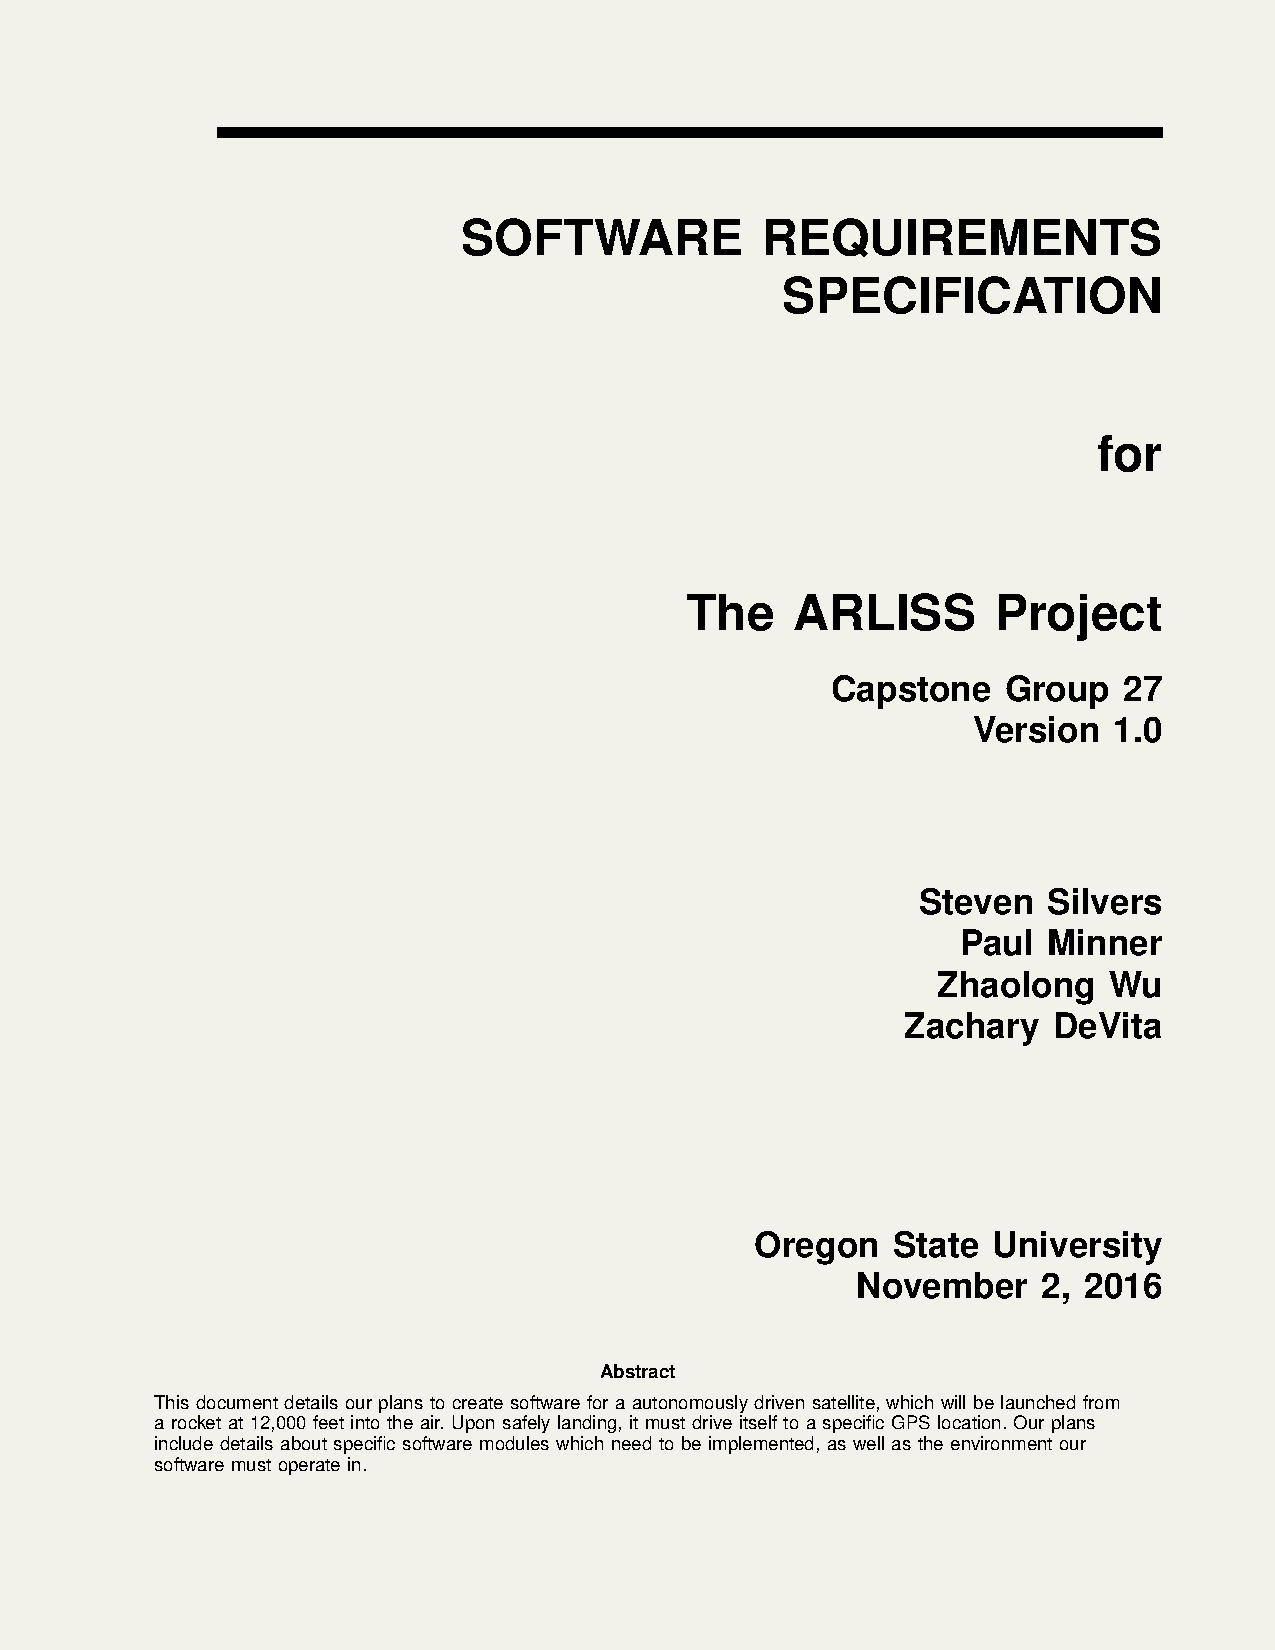
\includepdf[pages={1-},frame,scale=0.90]{requirements/srs.pdf}

\subsection{\textbf{Revision History}}



\section{\textbf{Design Document}}
\subsection{\textbf{Original Document}}
The following document is the original version of our team's Design Document. The Design Document describes each software component in detail. This includes the purpose of each component, how it is being implemented, and how the components interacts with one another.    
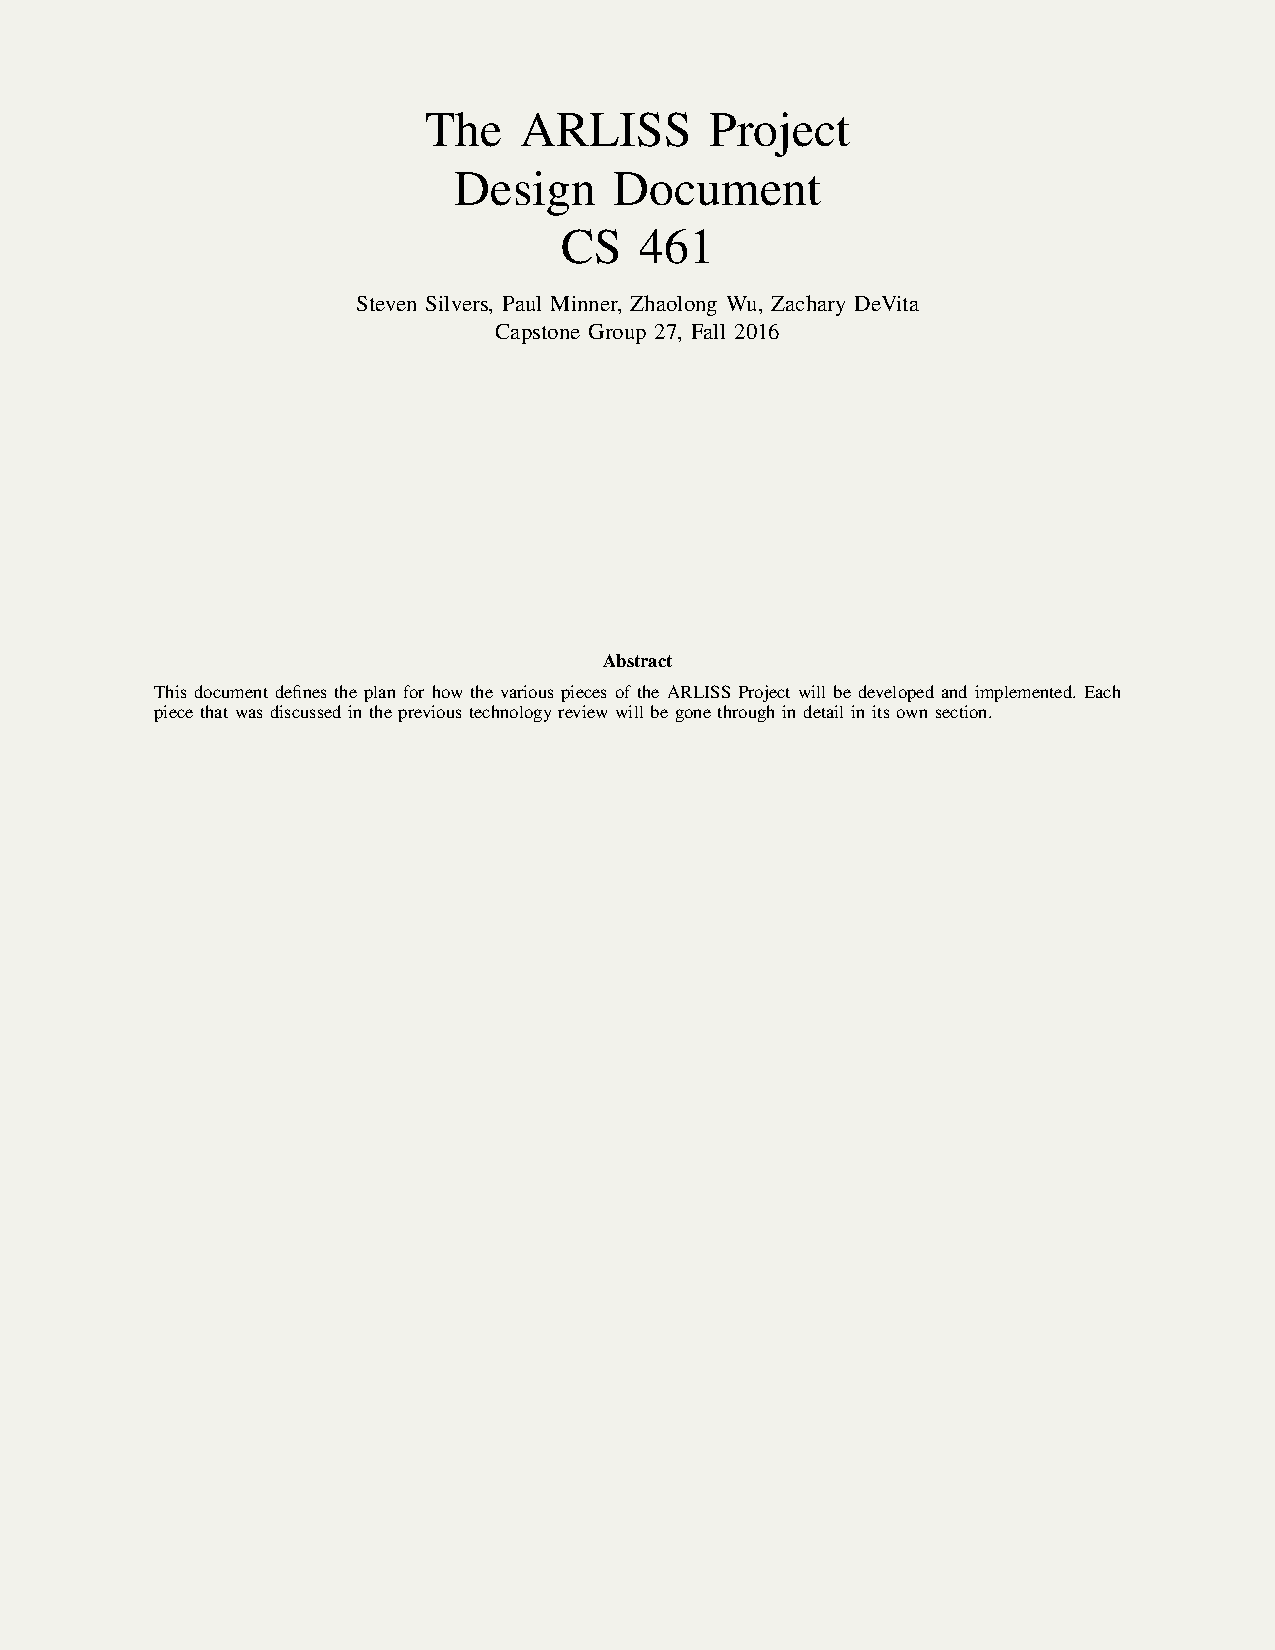
\includepdf[pages={1-},frame,scale=0.90]{design/design_original.pdf}

\subsection{\textbf{Revision History}}



\section{\textbf{Tech Review}}
\subsection{\textbf{Original Document}}
The following document is the original version of our team's Tech Review. The Tech Review was a research-driven document where we divided up the entire project into twelve software components and analyzed them. Each member of the team analyzed three components of the project by comparing and contrasting three alternate methods for implementing each of the compenents. At the end of each analysis, and based on the research, one of the three methods for implementing the component was chosen. 
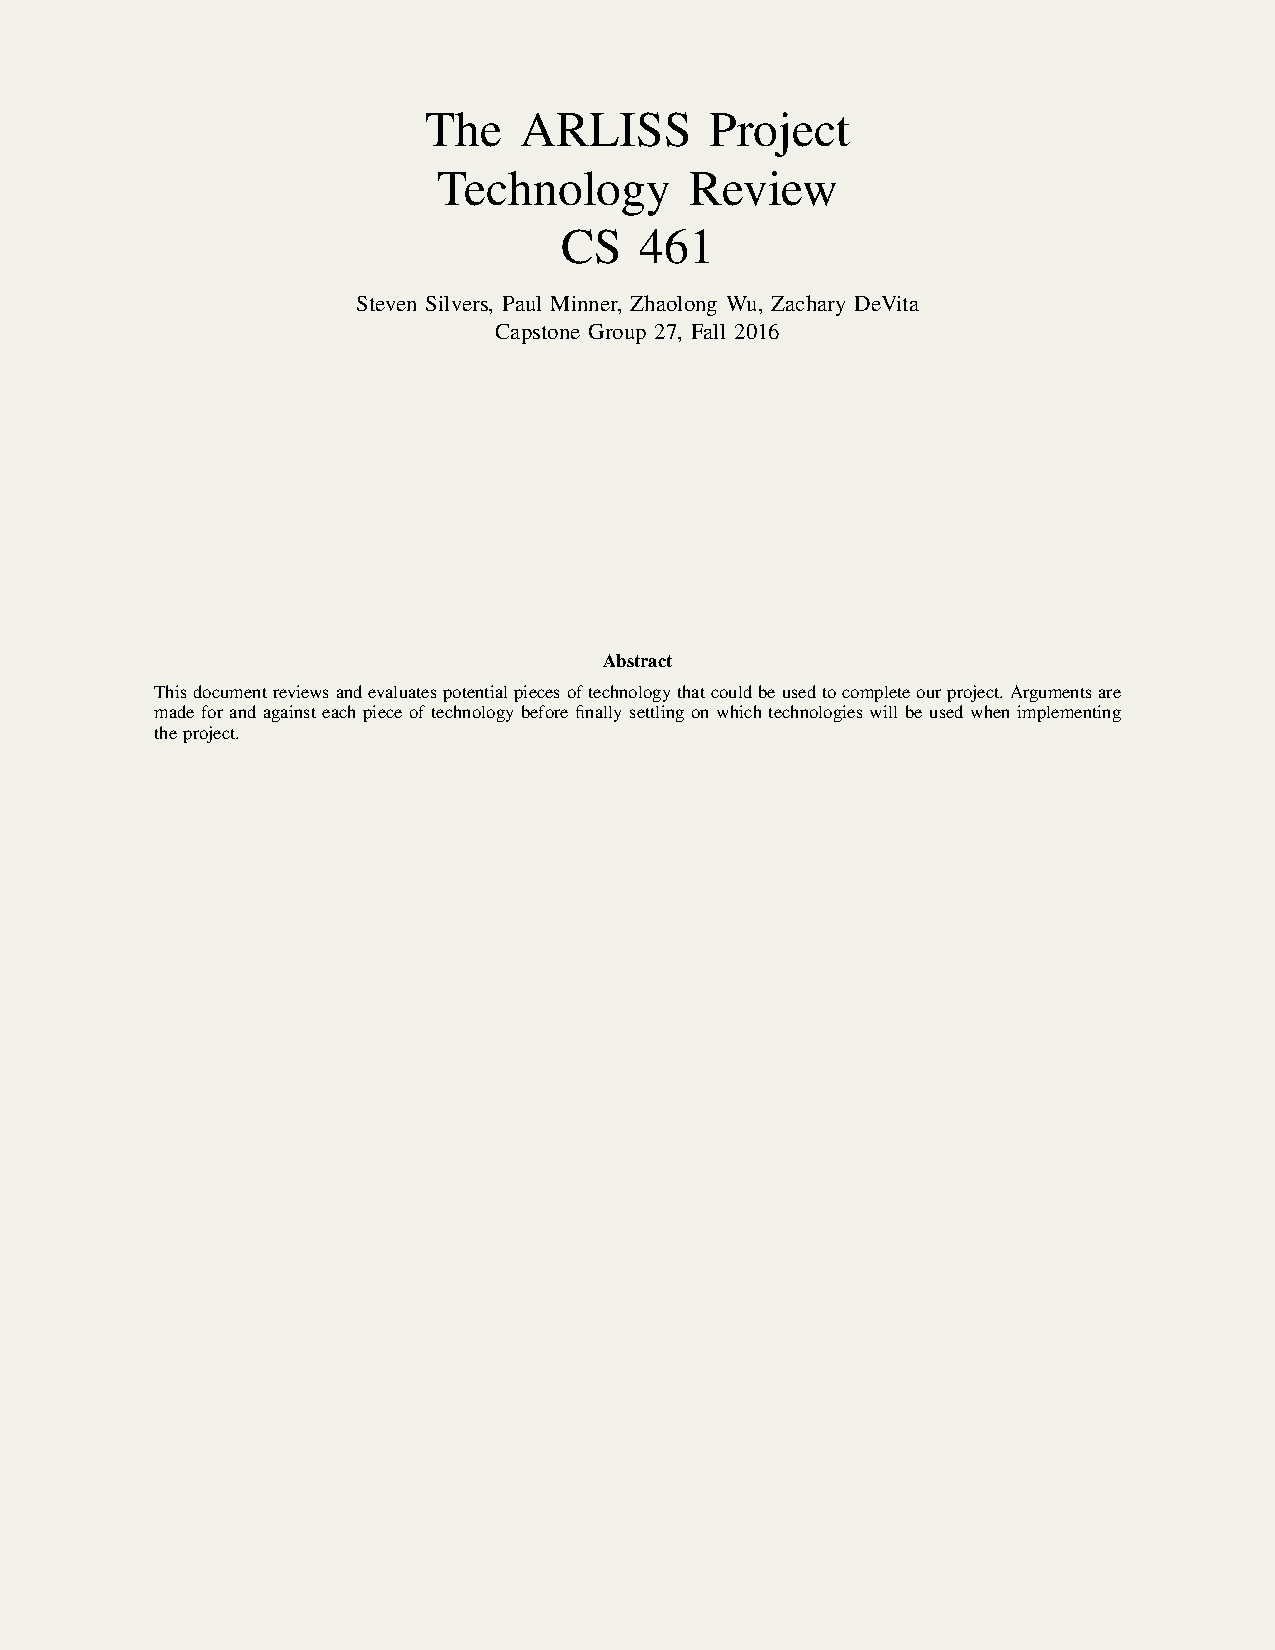
\includepdf[pages={1-},frame,scale=0.90]{tech/tech_original.pdf}

\subsection{\textbf{Revision History}}



\section{\textbf{Weekly Blog Posts}}
For the duration of this project each team member kept a weekly blog which was updated with individual progress, problems which were encountered, plans for the following week, etc. This section of the document will contain all weekly blog posts for each team member during the project. The blog entries will be organized by term, then by week, and lastly by the team member.
\subsection{\textbf{Fall Term}}
\subsubsection*{\textbf{\\Week 3}}
\paragraph*{Zachary DeVita -\\}
We just met with the entire team of engineers in our group Tuesday evening for the first time. This essentially just validated what we thought we were doing for our project already. We are working with a sub-team of mechanical engineers as well as a sub-team of electrical engineers to design a soda-can sized "satellite" which will eject from a rocket at 12,000' AGL and land safely on the ground using a parachute. This satellite, payload, robot, or whatever you want to call it, will then drive autonomously to a specific set of coordinates through some piece of the Nevada desert.\vspace{.3cm}
\par
Progress? Nope, no progress. We just met with our entire team for the first time, and our team of computer scientists have yet to even meet with out client. We have requested a couple extra days to wrap up our first assignment for the course, the 'Problem Statement'. Most of the assignment is finished, it just needs to be revised once to make sure the material is cohesive, and then put into a Tex based format to be submitted.\vspace{.3cm}
\par
Problems encountered would be that our project is so undecided upon, ambiguous, that it makes it absurd to write a problem statement at this point. Aside from that, we haven't been able to set up any kind of group meeting with our client. Our client is completely leaving all decisions made for the project up to us which is great for the most part, and makes communications between us less necessary, but it seems like there might be some important information that would be pertinent to the problem statement.
\paragraph*{Paul Minner -\\}
This week, we had our first meeting with every member of the ARLISS group. ARLISS group meetings will be Tuesdays from 6:30 - 7:30 PM from now on. At the meeting, we learned that our can satellite will be a rover which has to maneuver to a specific destination after landing. Until next meeting, we need to think about how this can be done, such as what kind of obstacles the rover needs to be able to go around and what sensors we will use for the robot's "senses".
\paragraph*{Steven Silvers -\\}
This week we met for the first time as a group and made contact with our client Dr. Squires. We are currently working on the problem statement document as well as getting our github group setup. A problem that we currently face is that our problem is very open ended, and also depends on the work of two other capstone groups at OSU.
\paragraph*{Zhaolong Wu -\\}
This Tuesday, ARLISS Micro Satellite Project group had the first weekly meeting, we have 10 people on board, from ME, ECE and CS departments. In order to fit everyone's schedule, we proposed to have every Tuesday 6:30-8:00 our official meeting time throughout this fall term. The ME team presented us the main idea of this project. The project will have two options to develop with, MISSION or Rover, it appeals to me more that we will go with the Rover option because it seemed more fun and challenging, until next meeting we will need some ideas in the Computer Science perspective that how conquer it.

\subsubsection*{\textbf{\\Week 4}}
\paragraph*{Zachary DeVita -\\}
We just met with the entire team of engineers in our group Tuesday evening for the first time. This essentially just validated what we thought we were doing for our project already. We are working with a sub-team of mechanical engineers as well as a sub-team of electrical engineers to design a soda-can sized "satellite" which will eject from a rocket at 12,000' AGL and land safely on the ground using a parachute. This satellite, payload, robot, or whatever you want to call it, will then drive autonomously to a specific set of coordinates through some piece of the Nevada desert.\vspace{.3cm}
\par
Progress? Nope, no progress. We just met with our entire team for the first time, and our team of computer scientists have yet to even meet with out client. We have requested a couple extra days to wrap up our first assignment for the course, the 'Problem Statement'. Most of the assignment is finished, it just needs to be revised once to make sure the material is cohesive, and then put into a Tex based format to be submitted.\vspace{.3cm}
\par
Problems encountered would be that our project is so undecided upon, ambiguous, that it makes it absurd to write a problem statement at this point. Aside from that, we haven't been able to set up any kind of group meeting with our client. Our client is completely leaving all decisions made for the project up to us which is great for the most part, and makes communications between us less necessary, but it seems like there might be some important information that would be pertinent to the problem statement.
\paragraph*{Paul Minner -\\}
This week, we met with the whole group and discussed the specifics of the rover. Next meeting, we should know exactly what the rover is going to be. We also got our Problem Statement document finished and turned in. Next week, we plan to meet the whole team to finalize our rover design, update our problem statement document, and write our requirements document.
\paragraph*{Steven Silvers -\\}
This week we turned in our initial draft of our problem statement and met with the ME and ECE teammates who are also working on the project. We are looking to figure out a definite timeline for completion of the hardware for the project so that we can plan out the software development.
\paragraph*{Zhaolong Wu -\\}
The team gathered together on Tuesday during the weekly meeting, we have narrowed down some possible approaches for this autonomous target finder vehicle, an air drone/glider UAB approach or a rover. We analyzed the pros and cons for both approaches. Air approach will involve power supply issues, as well as the software complex level. Ground approach seems is the best way for now due to the possibility of getting it working, but there are still some issues of it, for instance how to get over oversized bumps or so. Speaking on the software aspect, we still don't have too much ideas of how we are going to do it. All I can think now is we might need to use some types of sensors, and use some existing libraries and algorithm such as OpenCV sor so.\vspace{.3cm}
\par
Next week All team together we will make the final decision on which direction of approach we will use.

\subsubsection*{\textbf{\\Week 5}}
\paragraph*{Zachary DeVita -\\}
This week our team wrapped up the Problem Statement assignment, and worked on our rough draft of the Requirements Document. Communication in the group seems to be adequate enough to get our tasks finished on time so far, which is good. We have met with our extended team this week as well. The only real challenge that we encountered is in the description of our assignments. Some of the assignment descriptions seem vague and incomplete which has created a continuous need for clarification. That, and the fact that we can't possibly have a legitamate set of requirements because the hardware and design for our project hasn't been created yet.\vspace{.3cm}
\par
There isn't much to describe about our project at this point; everything is in the air. There is no way for us to be certain of the hardware we will be working with, or how the design of the ROV will look. Plans for the coming week are going to include finishing the final draft of the Requirements Document, or at least a "final-of-the-first-revision." This document is a evolving document, but a final draft of the initial revision will be completed this week.
\paragraph*{Paul Minner -\\}
This week, we revised our Problem Statement, and wrote our rough drafts for our Requirements Document. We also met with the entire group Tuesday night. We have now decided the rover is going to be a ground based tread design, as opposed to wheels or a flying design. We still don't know the specifics of the sensors, though. This means our requirements documents will be vague, and need to be revised when the sensor specifications are decided. Next week, we will meet will the whole team again to discuss more specifics of the rover, and write a final draft of our Requirements Document, as well as create a Gantt Chart for the rest of the year.
\paragraph*{Steven Silvers -\\}
This week we met with the ME and ECE teams and determined what approach we wanted to take with the rover design. As a CS team we wrote a rough draft of our requirements document to be turned in Friday. Our plan for next week is to revise the requirements document, as well as meet with the ME and ECE teams again.
\paragraph*{Zhaolong Wu -\\}
This week we were mostly working on the requirement document. During the weekly meeting we voted to develop a ground based vehicle. So now we have a general direction to go with, as the CS team we provide data communication between ECE and ME, so we are now waiting on the ECE team to finalize their selection of electrical parts then we will hopefully in next two weeks get a basic software structure.

\subsubsection*{\textbf{\\Week 6}}
\paragraph*{Zachary DeVita -\\}
This week was working primarily on the requirements document. I modified the previous latex template to include a table of contents. Finishing the formatting on this was a small victory. I had to manually change many of the defaults that were used in the 'IEEETran' document class which turned out to be a nightmare when you are simultaneously using the 'babel' package. There were very obscure and specific workarounds that were necessary for this combination of styling which made in extraordinarily difficult to change the numbering scheme on the table of contents and the section titles. When the document was done it looked amazing though. Everyone on the team pitched in, did their part, and the document came together and was turned in on time. Our extended team, including the mechanical and electrical engineers, did not meet this week. It seemed unnecessary to meet at this time, and many people had midterms this week. We met with our mentor this week, on Monday, to discuss the project and upcoming projects as well. As a team, we briefly discussed next weeks project. Next week we will be working on the technical review. This may be the most influential assignment we complete this term because it should help us determine the final design and framework of our software.
\paragraph*{Paul Minner -\\}
This week, we finished the Requirements Document. The entire ARLISS team did not meet today, but the CS group did meet to discuss changes which needed to be made to the Requirements Document. We met with our advisor on Monday, who told us our Requirements Document looked good so far. We each then completed a portion of the document over the course of the week, and on Friday, met to make minor changes and get the paper turned in. We met with our mentor to get the document signed as well.
\paragraph*{Steven Silvers -\\}
The plan for next week is to work on the technical review as well as meet with the ME and ECE teams to learn about what progress they have made. Since last week we have finished our requirements document and have began researching autonomous driving systems. One problem I have personally encountered is that I have been sick on and off since the beginning of week four, which makes finding time for capstone plus two other courses difficult.
\paragraph*{Zhaolong Wu -\\}
During this week we spent the most of the time on finalizing the requirement document, setup some early goals. The Tuesday meeting is cancelled so we didn't get the chance to talk with ECE and ME team. Next week the ME team will start developing the project physically so we will have more specs on the hardware hopefully start thinking about the actual implementation.

\subsubsection*{\textbf{\\Week 7}}
\paragraph*{Zachary DeVita -\\}
This week our team worked on the technical review for the class. Our team brainstormed 12 different topics to be covered in the technical review, and then split them up so each person was assigned three to write about. I personally reviewed the three most common languages for programming micro-controllers. This was an interesting review, and I learned a lot. This review put C++ on the map as a possibility for a language, and it may even help to determine some of the hardware components we request for the project, i.e. a 32-bit controller. I also compared and contrasted different sensors and systems used for object recognition. From the research I have thrown out photoelectric sensing as an option, and I was able to determine that ultrasonic radar in combination with CMOS imaging sensors would create the best system for the environment we will be operating in. The last topic of mine is comparing methods of recognizing the pole that must be bumped at the end of the expedition in order to finish. We did not meet with our extended team this week either. They had nothing new to share with us. We did meet with our mentor this week to discuss the technical review. Issues we are having would be that we still have not the slightest clue what hardware we will be working for, so every assignment we do in this class in comprised of educated guesses. I guess it is still better to think about these things than not, and maybe this experience will help us to make better decisions on what hardware our team does decide to go with. Next week is the design document. We haven't really talked about this assignment as a group yet, but I'm sure the time will come tomorrow. Hopefully I can get a good start on the poster next week as well.
\paragraph*{Paul Minner -\\}
This week, we just worked on the Technical Review Document. There was no meeting with the entire group this week, because the other groups didn't have any new information to talk about. Our CS Team did meet to discuss which pieces each of us would write about for the technical review. On Thursday, we finalized what everybody was going to write about. Next week, we will have a meeting with the entire group, and hopefully we will get more information about the types of sensors the ECE team would like to use. We will also start work on the Design Document. Some problems we're having right now is being sure the information we include on the Technical Review will be correct, because some pieces are also up to other teams.
\paragraph*{Steven Silvers -\\}
This week we developed our Technical Review document. We did not meet with the other subteams for the project because they had nothing to discuss with the group as a whole. We met as a group on a couple occasions to go over the plan for the technical review. Our plan is to look towards the next document for the class. I would also like to start discussing tasks for winter break so that we are ready to start at the beginning of winter term. The biggest Problem is that it appears we have conflicting timelines with the ECE and ME teams. Our work is dependent on what they develop, however we cannot begin some of the larger pieces of our software system without knowing what we will be working with.
\paragraph*{Zhaolong Wu -\\}
This week, we mainly worked on breakdown this project into many(12) pieces, and each of the team member has picked 3 pieces to evaluate the possible implementation methods, pros and cons. To build up the tech reviews document. Next week, we are going to start the first part of the implementation, the design document. It should be fun.

\subsubsection*{\textbf{\\Week 8}}
\paragraph*{Zachary DeVita -\\}
This week our team focused on finalizing our technology review, and managed to get that turned in early in the week and on time. Aside from finishing the technology review, our team has begun working on the design document assignment. I personally have not begun writing any of the document, but I have started doing some preliminary research for the assignment. I believe the assignment should go relatively smoothly for myself. I do need to figure out what one of my topics could be; in my tech review I compared the 3 most commonly used languages for programming microprocessors, but I don't think this is an appropriate topic for a design document. That is something I'll need to speak with Dr. Kevin McGrath about. We met with our mentor this week, as usual, and he made it sound like we are on track and doing well. We also met with our extended team on Tuesday evening. They were able to give me a prototype CAD image of the satellite which will come in handy for the poster our team is making. They didn't have anything that was too pertinent to discuss, but they are speaking with the point of contact for the competition in hopes to get the precise specs for the satellite. That seems like an important step before we start building the satellite. Next week I, and the rest of the team, will be finishing up research for the design document and writing the final version. More meetings next week, and finishing the design document.
\paragraph*{Paul Minner -\\}
This week, we finished our tech review, met with the entire ARLISS group, and started plans on the design document. After meeting with the group, we now have a better idea of what sensors will be used, although we still aren't sure if a camera or sonar will be used for the obstacle navigation system, which is a problem for the design document's accuracy. Additionally, it was decided the GPS will be used to calculate altitude for the parachute deployment, which will now need to be changed in the tech review later. For the design document, we created a simple outline, as well as some ideas for what to include for some sections. Next week, we plan to focus on the design document. There should be another meeting with the entire ARLISS group next week where we will nail down what sensors will be used, and we will talk about how the different technologies will fit together for the design document.
\paragraph*{Steven Silvers -\\}
This week we worked on planning out the Design document and also submitted our Tech Review. The plan for the following week is to work on writing the Design document as well as begin planning the progress report and poster. The biggest problem I see at the moment is Thanksgiving break cutting into work time.
\paragraph*{Zhaolong Wu -\\}
During this week, we, three teams finally gathered together and discussed the detailed design, the ME team has the basic dimensions specs done for the ECE team, so that they have an idea of what components to use in order to fit into the CanSat, we settled we are going to have a 9V 1200~1500 mA battery for the main power supply, two servos, two motors(brushless or brush), GPS modules for the CanSat. I'm still doing researches on whether we are going to have a camera/SONAR/RADAR for the obstacle detection, as well as if a accelerometer or a compass is needed to enable the autonomous feature.\vspace{.3cm}
\par
Next week, we will mainly focus on the design document and the end of term presentation.

\subsubsection*{\textbf{\\Week 9}}
\paragraph*{Zachary DeVita -\\}
This week was spent working on the design document. I managed to finish up my sections of the design document early and am currently done. I formatted the latex for the document using the requirements for the assignment as a guideline and posted it on github for the other members to add their sections. Our team as a whole should be wrapping up all their sections this weekend as well so that we are able to get a running start on the progress report assignment. Our team met with our mentor, as well as, the extended team of engineers this week. Not too much new information to speak of. A note for next week, I need to speak with the extended team and get some much needed information. It is time that our team knows the exact requirements for the competition and what sensors we are using. The extended team needs to have these defined in order for us to effectively accomplish our assignments, and, so far, it has not been that way. The assignments are getting incredibly difficult without this information now that we are getting into the specifics of design. Next week we will be working on the progress report, and hopefully the presentation as well. This is an absurd amount of assignments to all be due in such close proximity of time. Hopefully our planning ahead will pay off in this regard though.
\paragraph*{Paul Minner -\\}
This week included Thanksgiving, so our group didn't meet much this week. There was a meeting on Tuesday with the whole group, but I was unable to attend this week. We did manage to finish the majority of the Design Document this week, though. Each group member worked on the same pieces as we did for the Tech Review. Next week, we plan to finish the Design Document, and finish the majority of the final progress report. Some issues we have had is being sure if we will actually stick to the design document, because some decisions are difficult to make without any testing to see how well it works. For example, the algorithm to get the rover unstuck from obstacles may change if we find that the algorithm we thought of doesn't work very well.
\paragraph*{Steven Silvers -\\}
This week we finished our design document. We decided to get it done early giving us more time to plan and work on the Progress Report as it seems that the Progress Report will require a but more work. The plan for this week is to layout the progress report design and also to decide what we will do for the video presentation portion. The only problem I foresee is being able to manage multiple projects over multiple courses all being due around the exact same time.
\paragraph*{Zhaolong Wu -\\}
This week, I mainly worked on the final design document, I went to the meeting on Tuesday and it was great to hear that the ME team have finalized the basic design motor, motor selection, the ECE team are ready to purchase some sensors. We decided that we will use the Raspberry Pi zero and make the microprocessor. Mean while, we still need to figure out how to make the tread.\vspace{.3cm}
\par
Next week will be the last week of this quarter, we will wrap everything up and getting ready for the next phase of this fun project!
\subsubsection*{\textbf{\\Week 10}}
\paragraph*{Zachary DeVita -\\}
Week 10 was a busy week indeed. Our team managed to finish the majority of our Design Document over the weekend so there was not too much time spent working on it. Everyone did there part and researched their topics, wrote up their portions of the document, and we managed to get it turned in on time. We also made sure to get a considerable head start on our progress report. I finished up my sections and the template for the progress report by Thursday or Friday so that I could focus on final projects in other classes, and the presentation for this class. So far everything has gone well, or a least worked itself out. We met with the rest of the team on Tuesday to discuss hardware in more depth than usual. Nothing too concrete has been chosen as far as hardware, but some ideas were thrown out. The electrical engineers apparently want to use an AtMega128 processor. I suspect that it is only because that is what they are accustomed to and not because it is the best tool for the job. Ideas for sensors were also mentioned. Hopefully they consider the CMOS and the ultrasonic sensors that I researched and suggested to them. We finally got the specifications for the competition. At least it is before we start implementing. Our team plans on putting forth some effort and working on this project over break which would be nice. I've requested some supplies from Dr. McGrath so that I can work on some of the coding over the break. Next week is finals, and I still go to finish up that presentation, but, other than that, I'm done.
\paragraph*{Paul Minner -\\}
This week we finished up our Design Document, and started working on our Progress Report and presentation. For the progress report, we decided to split the weeks up and each write a couple weeks. We still need to write the rest of the Progress Report. The Design Document we got signed by our mentor and turned in on time. We had a group meeting this week, where we discussed more specifics of how the different components of the rover would work. Over break, we will do more research how to implement our components, and begin working on them. Problems we face is we have to start writing code before we have the hardware which will run the code, so some code may change.
\paragraph*{Steven Silvers -\\}
This week we finished our Design Document and got it signed and submitted. We've begun work on our progress report, with the plan to begin recording the presentation over the weekend. At this weeks group meeting we had further discussion about the actual design and implementation of our rover, as well as brainstormed ways to best get out of the can once we have landed. The plan for break is to continue researching methods of implementation and various technologies, as well as starting to code framework for the project. This will be difficult as the ECE team still has not locked down what they will be working with hardware wise. Until the hardware has been figured out, it will be difficult to make any significant progress on implementing the software.
\paragraph*{Zhaolong Wu -\\}
It's the final week of this term, we had not to much in beside finishing up the design document and making the progress report and final presentation. We had a team meeting on Tuesday, mainly discussed some protocols we are going to use on the rover, as well as some test cases. Today the Mechanical Team got an email from the ARLISS competition committee, they sent us a detailed CanSat competition specs, we will start working on the actual implementation through the break, and hopefully will have a version 1.0 done by the midterm winter term.

\subsection{Winter Term}
\subsubsection*{\textbf{\\Week 1}}
\paragraph*{Zachary DeVita -\\}
Week 1 of winter term. I actually, and sincerely, worked on the project over break. Nothing too impressive, but I have a working program which converts a colored 24-bit .bmp image into a two-dimensional array of binary values. Essentially zeros in the array indicate that the change in grade of the terrain is safe to traverse, and that there are no obstacles present. This program needs some serious testing though, and I'm not certain how to create images that would accurately represent the terrain in Black Rock Desert. I have worked out about all I can without a proper way to test, but I think it is a good start to the most difficult part of the programming for our project. It seems that our electrical engineers have decided to choose an 8-bit AtMega128 processor for the project. This means we would be programming in only C so I spent some time researching how to mimic some of the C++ features that our team was hoping to utilize. Aside from this, it's the first week and our team hasn't even had a meeting so there's not much to write about.
\paragraph*{Paul Minner -\\}
This week, we started getting back into the swing of things. We've scheduled our weekly meetings with our TA for 11:30 AM Tuesday, and are currently getting our weekly meetings with the entire group figured out. Over break I researched about the components needed for the parts of the project I'm responsible for, such as GPS and cameras. Soon, we should begin actually implementing our design. Our only implementation problem is that the hardware isn't available yet, and therefore we will have to simulate it.
\paragraph*{Steven Silvers -\\}
Start of winter term, over break I studied various autonomous driving methods since that is the main part of the project I am responsible for. I also looked at different hardware implementations and how they would possible effect our programming decisions. We are communicating with the rest of the team to find a weekly meeting time, and have set our weekly TA meeting for Tuesdays at 1:30pm. Hopefully our whole team meeting time will be set soon so the ECE and ME teams can update us on their progress.
\paragraph*{Zhaolong Wu -\\}
The winter term kicks off this week, we had one class meeting and instructor McGrath officially announced that we are in the implementation phase of the capstone project, we setup the mentor meeting time on every Tuesday 11:30pm to fit every team member's schedule. We are still waiting on the new weekly team meeting time with the ECE and ME team, and we are going to talk with the client to let her come to the first team meeting to give us a general direction.\vspace{.3cm}
\par
During the winter break I spent handful amount of time on researching the autonomous driving vehicle especially on GPS works in it, hopefully we can get our first prototype done soon.

\subsubsection*{\textbf{\\Week 2}}
\paragraph*{Zachary DeVita -\\}
Not much to report for this week. We met with our mentor for the first time this term, and he gave us some due date info for the project. We are supposed to have a prototype for the project, a fully working program, written by week 5 which is comical. We still haven't met with our entire team which includes the other engineers participating in the project. We do have a time to meet with them next week so hopefully we will have something to work with at that point. Much of our programming requires interacting with hardware that is being used on the "satellite", but that hardware is being built by the electrical engineers. Their due date for finishing the hardware, which we must have in order to finish our programming and begin our testing, is approximately the same due date as we have to finish our programming. There seems to be a major flaw in how these multi-disciplinary projects are organized. I'm no rocket surgeon, but it would make infinitely more sense to have the senior design projects, which are cross-disciplinary, have their implementation terms staggered so that the hardware is being completed at the end of one term, and then the programming could begin in the subsequent term. Mind-blowing, isn't it.
\paragraph*{Paul Minner -\\}
This week, we haven't accomplished much. Mostly, we have started planning what parts need to be completed for the alpha build due at the middle of the term. The entire ARLISS team is working on setting up a time for group meetings. Currently, Wednesdays at 6pm - 7pm is thought to be the time.
\paragraph*{Steven Silvers -\\}
This week we met with our TA Franks for the first time this term, and discussed what is expected of the group as far as implementation of our project for this term. We as a group decided what a successful alpha version of our project would look like. We decided since the other two teams on our project would mostly likely not be finished with the hardware implementation until the end of the term that for our alpha release we would write simulators for our individual modules to demonstrate that they function properly. The goal for the Beta release is to have to code implemented on hardware, but that is entirely dependent on the progress made by the ME and ECE groups.
\paragraph*{Zhaolong Wu -\\}
During this week, we met our TA for the first time this term. We set the weekly meeting with him on Tuesday 1:45-2:00 pm, he mentioned during the meeting this week that the basic structure of this term in term of our project, we have two check offs, alpha version which will happen in midterm and beta version that I believe would be the final. So we suppose to have a functional physical prototype done by the midterm despite this is way beyond of our control because we have to get the ME team and ECE team to finish the actual rover then we can start to program it. So we have settled down that we will have something simulations done by the midterm, and each person in the group will be in charge with topics that we wrote in the tech-review from last term. We will have to send an email to the TA to specify though.\vspace{.3cm}
\par
Other than that, we didn't have to much, I'm still doing researches on my part which I believe that's what every team member is doing at this moment, we still have not met, or heard any people in the ECE and ME team yet, we hope we will do next week.

\subsubsection*{\textbf{\\Week 3}}
\paragraph*{Zachary DeVita -\\}
This week our team has decided on a microcontroller which means we know our processing speed, and which means we know which language we can program in. This came as great news as we can now begin our programming for the project. Our team will be writing the code for our project in C, and I have begun writing a program which manipulates images and detects the edges in the images. This utilizes the opencv library which is an amazing, powerful library. So far I have determined a method of converting images which eliminates the noise in the image, and that seems to be the most effective configuration of function variables for our purposes. I will attach images showing the progression. These include an original photo taken in Blackrock Desert and two different methods of eliminating noise which have shown success. There are many different methods of image manipulation which can be utilized for eliminating noise in the image. For both of the methods which I have found, I first convert image to grayscale, then I blur the image along the horizontal axis. For one image I then use the Canny filter to finish the process. On the other image I run it through a binary inverted threshold. Both these methods seem to accomplish what I am looking for so we might rely on testing to determine the best. Now I need to convert these images to a double binary array, or do I? The next step is kinda in the air. The original plan was to convert to a binary array, but I'm not sure if that is the most efficient method.\vspace{.3cm}
\par
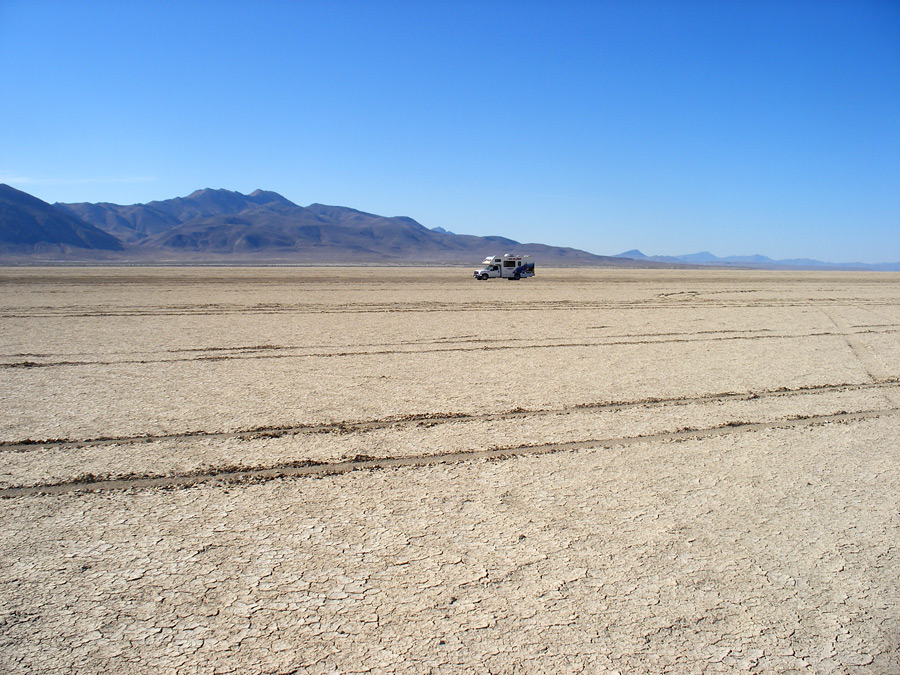
\includegraphics[width=12cm,keepaspectratio]{blackrock}\vspace{.1cm}
\par
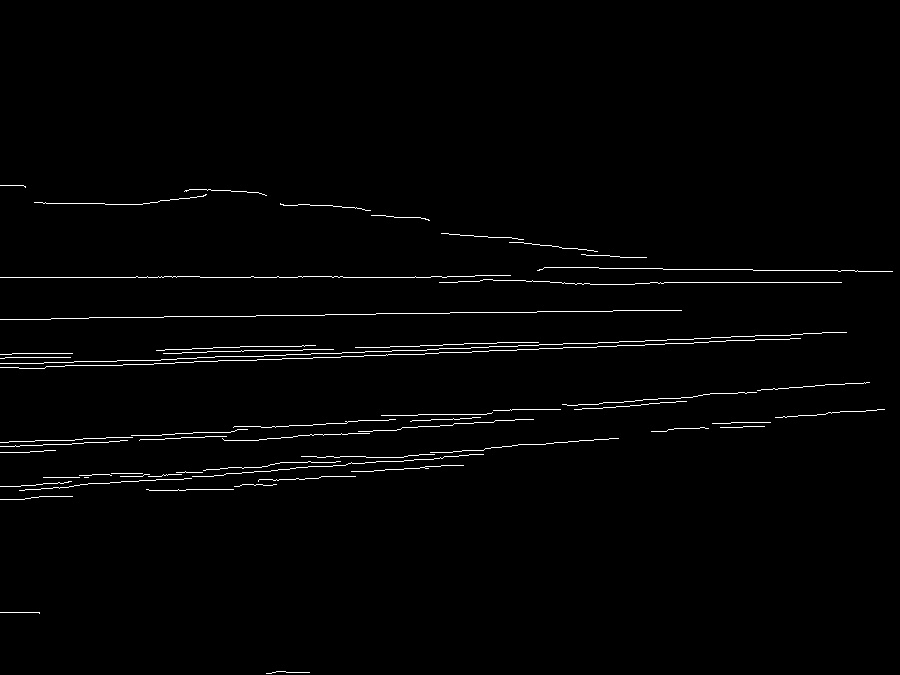
\includegraphics[width=12cm,keepaspectratio]{canny}\vspace{.1cm}
\par

\includegraphics[width=12cm,keepaspectratio]{thresh}\vspace{.3cm}\vspace{.1cm}
\par
Here's some other configurations of filters that might be considered as well. Neither of these use the Canny filter; one is blurred, and the other is not blurred.\vspace{.3cm}
\par
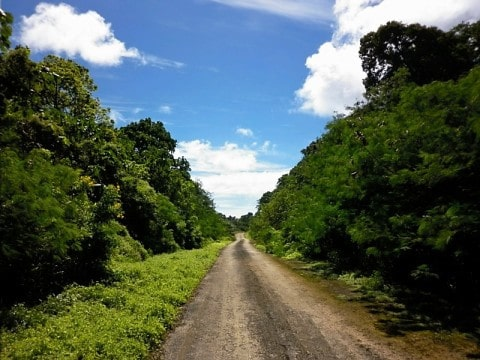
\includegraphics[width=12cm,keepaspectratio]{road}\vspace{.1cm}
\par

\includegraphics[width=12cm,keepaspectratio]{road2}\vspace{.1cm}
\par

\includegraphics[width=12cm,keepaspectratio]{road3}

\paragraph*{Paul Minner -\\}
This week, we finally met with the entire ARLISS group. At the meeting, we discussed where each group was, and upcoming due dates. We also finally know exactly what hardware we will be implementing our software on, which is a Raspberry Pi Zero. Each member of our group has been working on implementing their portions of the project, and will continue to do so next week. There should also be another large group meeting next Tuesday to discuss progress with the other teams. One issue we are running into is simulating our software. Some components are difficult to simulate, which means we won't know exactly how the software will react until the hardware is finished and we can test the rover itself. Other than that, simulating most modules of our software for the alpha build seems doable.
\paragraph*{Steven Silvers -\\}
This week we held a team wide meeting with the ECE and ME groups to better figure out timelines and what everyone is working on. It sounds like the ECE team has finally settled on using a Raspberry Pi zero as the main board for the rover, giving us a better idea of how we need to implement our code. Progress has continued to be made on developing and simulating our individual code pieces in preparation for the week 6 alpha release.
\paragraph*{Zhaolong Wu -\\}
We finally had the first all major groups together meeting this week, we set the weekly meeting time on Tuesday from 6-7pm. The meeting went very well and it was surely very informative for our computer science sub-team, the mechanical team told us the specs of the rover design and what there schedule looks like for the winter term, just like us, they also need to have a working version of prototype to be done by the week 6, the working version means the rover has to be ready to be tested, under basic functional requirements. For example, being able to drive from given waypoint A to B, driving around a circle, etc.\vspace{.3cm}
\par
We split work for now to the alpha version release, Zach is going to continuing working on the camera, Zhaolong is going to work on how to use GPS data, Paul is going to work on the parachute deployment and Steven is going to deal with the board.

\subsubsection*{\textbf{\\Week 4}}
\paragraph*{Zachary DeVita -\\}
Our team met with our mentor and our client this week. Our client showed up at our team meeting which was very beneficial. We were able to get some of our questions answered by here. We also were able to decide on some important stuff at the meeting regarding hardware we will be working with. We now know all the hardware which we will be interacting with! We had a class lecture this week as well. We were given a description of our mid term progress report and some details of the assignment. As far as progress on the project, I have finally been able to get in contact with Bill Smart who is one of the leading researcher in robotics and machine learning here at OSU. He has put me in contact with some of his researchers so that I can get some assistance working on the object detection algorithm. I have yet to hear back from them, but gaining his input and assistance is a huge step in implementing our object detection. The alpha version requirements of our capstone projects has been defined by Kevin McGrath. His requirements make it seem far more plausible to have completed by week 6.
\paragraph*{Paul Minner -\\}
This week, we've continued to work on the alpha release of our project. This consists of creating the modules for each section of the journey, and simulating the input from the sensors to make sure they work correctly. We also got our OneNote page set up. We still need to revise our documents to reflect recent changes in our plans, and we need to write our progress report.
\paragraph*{Steven Silvers -\\}
This week was mostly business as usual, we continued working on the alpha version of our project, as well as had an all group meeting that included our client Dr. Squires. My development module has been changed in that it will be getting a .mat file as input instead of a 2d binary array. This change will need to be reflected in the requirements document.
\paragraph*{Zhaolong Wu -\\}
This week we had 2 major parts going on, during the all group weekly meeting, the ME team leader Kyle laid out the projected expense, as well as how much for now to make one single rover, which is roughly about 299 dollars. As the CS team for now we just need 2 Pi Zeros and one camera. Our client Dr.Squires showed up as well. We discussed some details of the CanSat competition, like what the target pole looks like in order to program the vision system. Per competition rule the rover need to have the GPS coordinates recorded in a time interval, which is fairly easy task, we are planing to put a little script in our program that let it create a log file automatically at the end.\vspace{.3cm}
\par
During Thursday's class meeting, both instructors went through things we need to do in the future of the term, I'm aware that first we need a team leader, due to the over crowded classroom and the time conflicts with another class, I wasn't able to find the team members and had to leave class early, I will send out an email to ask.

\subsubsection*{\textbf{\\Week 5}}
\paragraph*{Zachary DeVita -\\}
This week our team met with the other engineers for our project and with our client on Tuesday. We had some new assignments come up for the class this. One of the assignments is the progress report. Our team needs to update the original document with what each of us has been doing for the last five weeks of the term. We also need to make another presentation for our project which will be approximately 30 minutes long. We are also updating our documents from last term with any necessary changes and publishing them on a OneNote notebook. This week I created the OneNote notebook for our project and I've been working with some of Bill Smart's graduate students to develop a machine learning algorithm for locating the pole at the end of our satellite's trek. These types of algorithms are pretty foreign to me so there will be no way that it gets finished before our alpha release but hopefully for our beta release. I've been doing a lot of research on machine learning object recognition and it is extraordinarily interesting to me. I hope I am able to get this chunk of code working.
\paragraph*{Paul Minner -\\}
This week, we made significant progress on our modules in preparation for the upcoming progress report and demo. I finished the Parachute Deployment Module, as well as the Getting Unstuck From Obstacles module, with testing programs for each module. Our current plan for the alpha release is to run each module as a separate program being tested with simulated input from the GPS and Camera. Our main problem is some pieces, like converting the image to binary, is difficult to know if it will work correctly until we can use images that are closer to the images the camera will take during the competition. For the alpha release, we aren't worrying about this, though, and are just attempting to have each module work to some degree. Next week, we plan to write up our progress report and demo our alpha release.
\paragraph*{Steven Silvers -\\}
This week was spent doing work on the alpha version of the modules I am responsible for, mostly the obstacle avoidance system. Because of this modules complexity it was decided that the alpha would be a lower level "prof of concept" and full functionality would be added by the 1.0 release. I edited both the tech review and the design document to reflect changes that had been made to the project for the sections I am responsible for. The biggest edit was for the control board, as the ECE group finally settled on what board they would be using and it was not what the document said would be used.
\paragraph*{Zhaolong Wu -\\}
This week we were mainly focus on revising the design document and get the mid-term assessment ready. I'm still trying to test the gps functions like feed dummy data in and trying to see the systems response. Also I did some researches only and wrote a obstacle detection pseudo code. Next week we will finish up our progress report and get more testing done.

\subsubsection*{\textbf{\\Week 6}}
\paragraph*{Zachary DeVita -\\}
This was a busy week. Our team spent the entire week wrapping up our presentations, middle of the term progress reports and updating our documentation. I believe the only documents our team needed to update were the Tech Review and the Design Document. I had to change pieces in both of these documents; anything referring to us using the ultrasonic sensor had to be removed. My updates were completed at the beginning of the week, as well as, most of the formatting for our team's OneNote. This allowed me to focus on the progress report and the presentation. My section of the presentation ended up being just over 7 minutes which was the expected length for each of our team member's parts. Everything got done just in time to turn in on Friday. Steven concatenated each of the presentation pieces, and I uploaded the finalized documents to the team's OneNote.
\paragraph*{Paul Minner -\\}
This week, I finished up the find and touch the finish pole module, so all programming I need to complete for the alpha release is done. I also worked on writing the progress report and presentation. Everything is going smoothly, and we should be able to finish our alpha release by the due date.
\paragraph*{Steven Silvers -\\}
Week six was focused entirely on the upcoming alpha release and progress report. We decided that each team member would write their pieces individually and then combine them into one document Thursday, giving us plenty of time to submit the report on Friday. We got together with the ECE and ME teams for our weekly meeting, which ended early because all three groups were busy with progress reports and had nothing of significance to share. The ME team is uncertain of their capstone number, which hopefully they will figure out soon so that we can register as a group for Expo.
\paragraph*{Zhaolong Wu -\\}
During week 6, I spent most of the time to do more testing on the navigation system, the two output images above shows that the algorithm in the navigation program for getting the shortest path and initial heading, the output is matching the online GIS calculator. I'm currently waiting on to get the GPS, pcb board, and motor controller, etc. from the ECE team so I can do the integration tests. For the current testing method I used the location coordinates from the competition site Black Rock, NV, I hard coded two sets of coordinates as start point and finish pole.

\subsubsection*{\textbf{\\Week 7}}
\paragraph*{Zachary DeVita -\\}
This was a slow week for progress. Our team met with our mentor as usual, and our extended team had its meeting too. Much of this week was just discussion and planning for the last few weeks of the term. There was some discussion at our team meeting about the mechanical engineering requirements. It seems like they may need some basic driving functionality as one of their end of the term deliverables. I handed off the raspberry pi and other components to Paul so he could install the operating system on it and hopefully get the camera working. Paul also discussed merging some of the programming pieces together in the next couple weeks. We still don't have a finished ROV or the rest of the sensors and components to work with so we can only do so much. I asked the mechanical and electrical engineers for their team numbers so that I could register our team for expo. Hopefully they will know their numbers by next week. The current plan for the coming weeks is to start combining our individual programs together into a single program. My personal task is to finish the machine learning algorithm for locating the goal at the end of the ROVs expedition. I have been researching this, and working with Bill Smart's grad students to learn what I need to do this.
\paragraph*{Paul Minner -\\}
This week, we didn't get much new work done, but we have planned out our work for the rest of the term. At the weekly ARLISS meeting, we learned that the ME team will need basic drive from point to point functionality in the next two weeks. This means we will have to get a portion of our program installed on the raspberry pi and working. I now have the raspberry pi, and am planning to install an operating system on it this weekend so we can run our program on it. After getting basic functionality working, we will have to combine all the pieces of our program together and test the program as a whole. Still, our problem is we can now test on the pi, but we don't have access to the sensors and motors that the completed rover will have, so testing on the pi will really just show us if our program is too computationally expensive or not.
\paragraph*{Steven Silvers -\\}
Week seven I took a little bit of time to catch my breath and recover from being sick after a stressful week six. We are still waiting on the mechanical and electrical teams to figure out their capstone group numbers so that we can register for expo. The plan for week eight is to begin integrating our individual modules into a single system and to begin testing our system on the Raspberry Pi Zero hardware.
\paragraph*{Zhaolong Wu -\\}
During week 6, I spent most of the time to do more testing on the navigation system, the two output images above shows that the algorithm in the navigation program for getting the shortest path and initial heading, the output is matching the online GIS calculator. I'm currently waiting on to get the GPS, pcb board, and motor controller, etc. from the ECE team so I can do the integration tests. For the current testing method I used the location coordinates from the competition site Black Rock, NV, I hard coded two sets of coordinates as start point and finish pole.

\subsubsection*{\textbf{\\Week 8}}
\paragraph*{Zachary DeVita -\\}
Not a lot going on this week. I handed over my computer vision software for the obstacle detection to Steven so he can merge the two softwares into one program. The ECE team is still waiting on some parts for the rover. The mechanical team has an acrylic frame, but hasn't got any progress getting any of the parts onto it yet. 
\paragraph*{Paul Minner -\\}
This week, I focused on getting the raspberry pi ready for testing with our software. I made sure the operating system was installed, and I started loading my pieces of the program onto it. The most important part to test is the camera related pieces to test how fast they are, but those aren't finished yet. Next week, all the pieces should be finished so we can test individual pieces and combine all pieces into a single program. Our only problem now is the fact that the camera is so low to the ground. We won't be able to detect objects and obstacles from very far away, so we are urging the mechanical engineering team to allow the camera to spring up so that it is further from the ground.
\paragraph*{Steven Silvers -\\}
I spent most of this week attempting to merge my obstacle avoidance module with Zach's imaging module, with little to no success. I think what could be causing the problem is Zach and I may have opencv configured in different ways on our workstations, which is preventing me from properly compiling his source without making major changes. I will be sure to discuss with him in the coming days to see what we can do to fix this problem. Parts are still coming in for the ECE team, at the last group meeting the servos had finally arrived that will be used for unpacking the rover from the payload. The ME team has a frame cut from acrylic, but is not yet assembled and last I heard from them they had not started on the wheel system yet. The plan currently is to have all of our modules working in a single system by the end of the term, and whether or not that gets implemented on hardware is reliant on the progress made by the ECE and ME teams in the coming weeks.
\paragraph*{Zhaolong Wu -\\}
This week we had a class meeting to do practice expo pitch and tone. Other than that, I worked on how to update the new shortest route if an obstacle is found and we have to avoid, as well as an servo arm function if the rover falls sideways. I'm still fussy on how the mechanical team is going to release the parachute, I mean what kinda of protocol and is there high level programming involved? Also I'm a bit fussy on the ECE teams controller setup, if they are making the pcb how we are going to call the motor and gps to enable those functions?

\subsubsection*{\textbf{\\Week 9}}
\paragraph*{Paul Minner -\\}
This week, I worked on getting the camera working on the Raspberry Pi. Unfortunately, Nobody was sure how to connect the camera to the Pi, so the camera connector got damaged. I've ordered a new Pi which should arrive Tuesday, but that set back testing on the camera. Next week, I plan to integrate all the individual pieces we have into a single program, although it won't yet include all pieces because some modules aren't yet finished. We are worried that once we test our program on the actual hardware, the camera will be too low and we won't be able to detect obstacles very far in front of us. In that case, we will either have to raise the angle of the camera, or lower the speed which the rover travels. Hopefully, this doesn't end up being an issue.
\paragraph*{Steven Silvers -\\}
I made quite a bit of progress this week, I managed to successfully install Opencv on Linux, port Zach's imaging module so that it would run on Linux and not just from Visual Studio and added functionality so that it outputs a .csv file that I can easily open and use with my obstacle avoidance module. The .csv file contains values of zero where there is empty space(safe to drive) and nonzero and sometimes non integer values where there are edges. I just need to make a few edits to my module that allows it to adapt to the size of the .csv file, read any nonzero value as "1" and leave the zeros as they are, and it should be ready to check against real images.
\paragraph*{Zhaolong Wu -\\}
This week, I did making a little program that using opencv library to identify the center of a shape, it is still buggy and I'm still trying to make it work, once it works I will upload the file to the github.

\subsubsection*{\textbf{\\Week 10}}
\paragraph*{Paul Minner -\\}
This week, I finished up my merged program of everybody's modules which I'm going to demo for the Winter Progress Report. It had a few bugs which needed to be fixed, and I updated a couple modules with newer versions. Unfortunately, the ECE team didn't finish their PCB board, so we will not be able to run our software on the completed rover by the end of the term. The rover should be done by Friday of finals week, though, so we should be ready to implement everything as soon as next term starts and everybody is back. Next term, we will have to do a lot of testing to make sure our software is ready for the competition.
\paragraph*{Steven Silvers -\\}
This week I finished combining the imaging and obstacle avoidance modules and began running tests of various images to make sure that the avoidance algorithm was reacting appropriately. Testing for this system will continue in spring term, as well as working on optimization as it currently takes a minute to run on a Raspberry Pi Zero which is too long for what we need. I know for certain there are a couple ways the code can be improved, there are a couple image filters being generated from testing that go unused, and a couple functions with multiple nested for loops can be merged into a single loop. I also laid the framework for the poster, as well as added information on my module to the poster. The only things still needed for the poster are a team photo, updated photos of the rover and of our image filters as well as a paragraph on Zach's imaging module.
\paragraph*{Zhaolong Wu -\\}
This week we finally heard from the ECE team, and they said they will have the PCB ready on Thursday of finals week, which makes our hope of having a moving rover complete impossible, we will hopefully have it next term so we can make the rover move!!!

\subsection{Spring Term}
\subsubsection*{\textbf{\\Week 1}}
\paragraph*{Zachary DeVita -\\}
This is the first week of the term so our team has yet to meet, and we haven't yet met with our client or mentor. We have decided on a meeting time for both our team meetings and meetings with our mentor this week. I know, over the break, Paul worked on optimizing the obstacle avoidance system so that it would be more efficient. I personally spent my break working on the traffic cone detection software. I developed a backup program to detect the traffic cone, in case the machine learning method fell threw. This method uses a series of image filters to locate the traffic cone based on both its features and its orange color. The problem with this method is primarily that each time the frame goes through a filter every pixel in the image must be iterated over, and this process requires many filters. While I spent the break writing this complex, backup method for identifying the target, I also continued to develop the optimal machine learning classifier. I have developed the most effective machine learning classifier, based on my vector file, using the LBP (Local Binary Patterns) method. The LBP method of training a classifier only takes a few hours where the Haar method takes more than a week, so the idea is that I would find the optimal settings for training using the LBP method and then use them for the the training using the Haar method. Right now I am training a Haar classifier based off the optimal settings from my testing and should have this completed and tested by next week!
\paragraph*{Paul Minner -\\}
This week, we set up the meeting with the TA, as well as the rest of the group. The group meetings will now be held Wednesdays at 11:00 AM. Some progress was made over spring break on the project. I worked on speeding up the obstacle avoidance system.
\paragraph*{Steven Silvers -\\}
This week we set up our weekly meeting times with our TA, as well as with the ECE and ME teams. We recapped where we currently are in the project, what we have left to do and how we plan to get it done. Paul informed me that he made the code optimizations to the obstacle avoidance module over break, and now it runs on the Pi Zero well within the needed time frame. The plan is to see where the ECE team is with their hardware at next week's meeting, so that we can best project when we can begin system testing.
\paragraph*{Zhaolong Wu -\\}
This is the first week of spring term, we had set up our TA meeting time and group meeting time, we are excited to finish up our project.

\subsubsection*{\textbf{\\Week 2}}
\paragraph*{Zachary DeVita -\\}
We met with the entire ARLISS team this Wednesday for the first time this term. No good news from them; the hardware is still not operating correctly. There are several mechanical issues with the prototype. The frame seems to be too tight against the wheels for them to turn freely and one of the motors does not work. This has been a tremendous setback for our team. Without the mechanical parts working, neither the electrical team or ourselves are able to do any testing on the rover, and we are beyond the point where we should have already been testing.\vspace{.3cm}
\par
As far as myself, I have finished training my haar, machine learning classifier. It took nine days, but I got a working, accurate classifier for identifying a traffic cone! I am able to determine the pixel location for the center of the cone is as well, which is necessary for Paul's algorithm to work correctly. I did run into some issues with false positives, which is almost impossible to avoid, but I used a feature from my previous algorithm to help verify my results. The classifier is a feature based classifier which uses geometry and shape patterns to recognize an object. When the classifier is made, all images which are used in training are converted to grayscale so the color of the object is not taken into consideration. Since the bright orange color uniquely identifies this object and is an atypical color to be observed in nature, I decided to verify results by checking that the color of the object is orange. I take a few points from the result, convert them to their HSV equivalent, and then ensure they are in the appropriate range of values observed on traffic cones. This method seems to work pretty well!
\paragraph*{Paul Minner -\\}
This week, the whole ARLISS team met for the first time. There, we learned hardware components of the rover still aren't working correctly. The frame is too tight against the motor so it won't turn, and the ECE team hasn't finished their PCB board yet, so the rover is still in pieces. This means we are still unable to do the testing we wanted to get done. I did get the rover though, and some of the motors are working, so I will start working on implementing the actual motor control functions into our program. Other than that, we have to wait until the rover is finished before we can do more testing.
\paragraph*{Steven Silvers -\\}
This week we got back on track with our meetings, and received a a prototype board from the ECE team so we could begin testing our our system on hardware. the ECE team is still a week or so out from having a finished final product which should give us enough time to implement before expo. There is also discussion of writing a separate demo script to run on the rover during expo. A draft of our poster is due Monday, we still need to take a group photo before the final submission.
\paragraph*{Zhaolong Wu -\\}
This week we met with the ECE and ME team on Wednesday, good news is Zach got the cone detection part working and showed off to everyone during the meeting! Bad news is ECE team had to redesign the PCB because the old one is too big and won't fit in the rover, they are going to have it ready by next week, also as the implementation goes they found that the motor has enough torque but not enough speed, which led the rover goes very slow, so we are going to replace some high speed lower torque rover, aside, one motor was jammed so we can't perform any testing on the rover. Expo has been signed up already.

\subsubsection*{\textbf{\\Week 3}}
\paragraph*{Zachary DeVita -\\}
The rover is still not fixed. The electrical team has still not been able to test all of their code. We still do not have a rover to implement and test our code on.\vspace{.3cm}
\par
I have improved my algorithm for detecting a traffic cone. I have made it so that when there are multiple results found, instead of throwing out the frame, I now check both results for orange and only discard the results if neither are orange. I also tested several additional methods of verifying results. I tried to also implement a check for the white band, but it seemed that it was severely cutting down the rate that any results were returned, so far more false negatives. I am considering a method were I use image filters and convex hulls to verify the data, but this method would use considerable more resources to run.\vspace{.3cm}
\par
I made a little improvement on the obstacle detection algorithm. I added a morphological opening to the series of filters which has helped to remove additional noise from the image.
\paragraph*{Paul Minner -\\}
This week, we've still been waiting on the other teams to finish the hardware of the rover before we can do more testing. I am currently working on adding the ECE team's motor control functions to our code so we are ready to start testing as soon as the other teams are finished. Unfortunately, we won't get to do nearly as much testing as we had hoped because the rover was supposed to be finished at the end of last term, but still doesn't work. Hopefully, next Wednesday at our group meeting we will have a fully functional rover to start testing.
\paragraph*{Steven Silvers -\\}
This week we met with Kirsten to get feedback on our poster, and worked with the rest of the ARLISS groups to figure out a timeline for finishing the project. It sounds like there won't be much time at all to test our software, as new motors had to be ordered and the ECE team is still waiting on a pcb to come in. It will be cutting it close for sure, but if all three groups stay on top of their tasks we should have a finished product by Expo.
\paragraph*{Zhaolong Wu -\\}
This week we are trying to finalizing our code, and still waiting on the ece team to give us a functional rover.

\subsubsection*{\textbf{\\Week 4}}
\paragraph*{Zachary DeVita -\\}
Nothing substantial to mention this week. Our team worked on the poster and got it finished. Our code was finalized this week as well. I know Paul spent some time combining some of the electrical engineering code with our code, but I didn't have anything to do other than working on the poster. I turned in my waiver for expo. We met with our mentor and the rest of the team this week. We still do not have a mechanically working ROV to work on. We still cannot implement our code or do any testing.
\paragraph*{Paul Minner -\\}
This week, we've worked on getting the repo ready for the code freeze and submitted our poster. I integrated some of the ECE team's code with our own so our code will theoretically work correctly on the actual hardware, although the only testing I have been able to do is to check if the motors move since the rover still isn't finished. The rover was supposed to be finished this week, but the GPS unit got fried, so now the ECE team is waiting for another one. Hopefully, we will get a finished rover soon so we can complete some testing before expo.
\paragraph*{Steven Silvers -\\}
This week we began organizing our repo to be ready for the code freeze on May 1st and also got our poster approved and submitted for printing. ECE and ME continue to have setbacks, the most recent being the ECE team fried the GPS sensor so now we need to wait for a new one. I don't believe the rover will be finished and fully tested by Expo, so we have started making plans for alternative ways to demo our software.
\paragraph*{Zhaolong Wu -\\}
This week we finalized our code and poster, we got the poster approved by both the client and instructors, and the poster is sent to the library to be printed for the expo! For the code part, mostly working but still no testing due to the ECE team's in-completion. The deadline delayed several times now and this will making us has a chance to not finish the whole project by the expo, I mean the actual rover, all the other code is done. The ece team still haven't written the servo function though!

\subsubsection*{\textbf{\\Week 5}}
\paragraph*{Zachary DeVita -\\}
Week 5... still waiting on the hardware. We met with our mentor and our extended team this week. The mechanical portion of the project still needs a bit of work. They still need to get a new frame made for the rover. Based on what the electrical team said at the meeting, they should have got the replacement GPS module in the mail by now, and it should have been installed on the rover by now. There is a motor that the mechanical team was waiting on as well.\vspace{.3cm}
\par
As far as my contribution, nothing substantial to report. I have been working with the algorithm for detecting the traffic cone, and I think I found a way to eliminate more of the false positives which we occasionally still get. We seem to occasionally get a false positive detected at points in an images where light is reflected directly into the camera. I have been working on increasing the size, i.e. number of pixels, of the minimum accepted result. These false positives in the image are so small that I can not make out any kind of cone shape or an orange coloration, so I believe enlarging the minimum accepted result will completely eliminate this issue.
\paragraph*{Paul Minner -\\}
The beginning of this week was spent getting the repo ready for the code freeze. I made a few small changes to the code and integrated the ECE team's device controller code into our own. I am unable to test if everything works correctly though, because we still don't have a completed rover to test with. Everything unrelated to the physical components of the rover we know works correctly, though. I also reorganized the repo so it is easier to tell what is our final product, and what is extra material. Other than that, we haven't been able to do much this week because all we're waiting on is testing, which can only be completed with a working rover. Supposedly, we should get a working rover next week, which won't leave much time for testing before expo.
\paragraph*{Steven Silvers -\\}
Still waiting on hardware to be finished by the ECE and ME teams, hopefully we can begin testing week 6 but at this point there doesn't seem to be enough time to implement and test the full system on hardware before EXPO. We have the code freeze and midterm report coming up, both of which shouldn't be problems.
\paragraph*{Zhaolong Wu -\\}
This week we had a meeting with the ME and ECE team, I'm aware that they still have not finished the rover, so we can't perform any testing yet. Within 10 days till the expo, we are just trying to get our parts work and do our best on the expo.

\subsubsection*{\textbf{\\Week 6}}
\paragraph*{Zachary DeVita -\\}
Still no rover. Spent this week completing the middle of the term progress report and presentation. We met with out mentor. We met with our entire team. We keep being told that we should get the rover in the next couple of days, but I don't know how much testing we would even be able to complete at this point. I am currently preparing for expo; at least we can still display some of our programming features at expo.
\paragraph*{Steven Silvers -\\}
We are having trouble getting in touch with the ECE team to see how the rover is coming. It looks like we should be getting the rover on the Wednesday before Expo, however we won't have enough time to integrate and test our software in time to demo it at Expo. I believe the plan is to have the ECE team write a small demo routine so that the rover will move around a bit at expo.
\paragraph*{Zhaolong Wu -\\}
One week from EXPO, our software is finished and ready to be tested, ECE AND ME team still haven't managed to put the rover together, at this point we are just going to show off our program on a laptop during the EXPO.

\subsubsection*{\textbf{\\Week 7}}
\paragraph*{Zachary DeVita -\\}
We finally got the rover this Wednesday. It was hot glued together and missing the camera so testing was still on hold. After a feeble attempt to get the camera installed on this hot glued mess, an sd card got fried, a wire became loose and the rover ended up back in pieces. Just before expo, on Friday morning, the rover had been re-assembled with a new sd card and the wiring fixed. There was still no camera installed, but at least the mechanical team had something to show. Expo went well; we had five or six people stop and talk to us. We had no industry people come anywhere near our presentation. I think this is due to the fact that we have red tags and were separated from the CS projects.
\paragraph*{Paul Minner -\\}
This week, we finally got a working rover on Wednesday, excluding a camera. We worked with the ECE team to try to get the camera working, but unfortunately, there wasn't enough room in the casing for the camera ribbon to fit. In the process of trying to get the camera working, the SD card on the pi was corrupted, so Simon and I worked with the ECE team trying to get our other SD card set up to run. We ended up not getting everything to work, and were unable to put our code on the pi. There was nothing we could do about this, though, because the only software we could demo at expo used the camera, and the ECE team couldn't mount the camera.
\paragraph*{Steven Silvers -\\}
The week of Expo, the ECE team delivered the rover to our team Wednesday night with the idea that we would mount the camera and begin testing. Upon receiving the rover, it was found that the camera port on the raspberry PI was completely blocked off, and there was no room in the electronics box for the camera ribbon. We returned the rover to the ECE team, who spent thursday working with the ME team trying to get something setup for the Expo demo. We already had our plan in place to demo our object detection with a laptop and a webcam so we are set for Expo.
\paragraph*{Zhaolong Wu -\\}
EXPO Week! Me and Paul worked with the ECE and ME team to trying to put the rover together, the rover was working on Wednesday but when we tried to mount the camera on we fried the SD card. It took us 2 days to make it barely working again, but somehow the rover stopped working again on the EXPO day, bummer. Now after the EXPO we are just trying to finishing this up and get ready for the competition.

\subsubsection*{\textbf{\\Week 8}}
\paragraph*{Zachary DeVita -\\\\}
\textbf{If you were to redo the project from Fall term, what would you tell yourself?}\vspace{.3cm}
\par
Zack... quit writing scripts for your presentations. It will make your presentation preparation take exponentially longer and it will sound exactly like you are reading from a script. Zack... more importantly, make those mechies get to work, and don't let them spend six weeks discussing the design. Also, try to get your hands on some kind of remote control car so that you can get some of the navigation and obstacle detection algorithms tested.\vspace{.3cm}
\par
\textbf{What's the biggest skill you've learned?}\vspace{.3cm}
\par
Computer Vision/Machine Learning/OpenCV. I can't decide; they're all so related and are such amazing skills. I have never been so inspired or felt so accomplished as I did when I got the cone detection algorithm working. The whole process of researching, designing, implementing, and testing, and without any direction or instruction made the experience truly incredible when I was able to succeed.\vspace{.3cm}
\par
\textbf{What skills do you see yourself using in the future?}\vspace{.3cm}
\par
I will absolutely be using computer vision, machine learning in my future; likely just for fun since the career opportunities related to computer vision seem to be rare. I also learned some teamwork skills. I have never had a group project anywhere near the size or duration of this so there was definitely some experience and some improvements gained in the area of teamwork and in my communication skills.\vspace{.3cm}
\par
\textbf{What did you like about the project, and what did you not?}\vspace{.3cm}
\par
I liked the idea of the project. Every aspect of the project, every individual component of the project sounds so interesting and fun. I loved the opportunity for inventiveness in the project, the freedom and creativity that came with the project. This project allowed for creativity and excitement which is something I have not been allowed to have in my other computer science courses. I love that I experienced all of the stages of software development. I like the feeling that I succeeded, on a personal level.\vspace{.3cm}
\par
I dislike that our project failed as a whole. I dislike that two of the teams deadlines were the same; I think ours was actually a week before the electrical engineering teams. I did not like the lack of expertise for our project. I was hoping a project like this would get me noticed and help me land that dream job, but now I just have a good response to the question, "What was a time you've dealt with failure." I also dislike confusing, incomplete and dynamic instructions for my assignments which seem to be the norm for these classes.\vspace{.3cm}
\par
\textbf{What did you learn from your teammates?}\vspace{.3cm}
\par
I learned that people may surprise you with their accountability. I have had few and far between positive experiences working with teams of students in my college experience, but I learned that, with good communication and clear expectations, people can and will get their work done. I guess I learned that communication might be the most critical factor in the success of a team.\vspace{.3cm}
\par
\textbf{If you were the client for this project, would you be satisfied with the work done?}\vspace{.3cm}
\par
This is a complicated answer. I don't think that I would be especially thrilled that the project never got completed. I would hope that I would recognize that there was no way that the computer science team could have implemented their components for the project when they never had a working rover to work on and test with. I think I would be able to recognize that the success of the project was completely out of the CS team's hands.\vspace{.3cm}
\par
\textbf{If your project were to be continued next year, what do you think needs to be working on?}\vspace{.3cm}
\par
I think the rover should be redesigned. Instead of having tracks it should utilize the traditional ARLISS competition rover design, with each end of the cansat being a wheel. After landing on the ground and right before it begins moving, it should have retractable spikes which shoot out of the tires. This would give the diameter of the wheel an extra inch which would eliminate the clearance problem. I think the computer science team should also get a chance to implement software on the rover next year. This would make it more likely to work, and give them a chance at the competition.

\paragraph*{Paul Minner -\\\\}
\textbf{If you were to redo the project from Fall term, what would you tell yourself?}\vspace{.3cm}
\par
I would try to establish better communication with the other teams. We only met the the ME and ECE team once a week, and that was usually the only time we would communicate about our progress. We also had a group text, but that wasn't used very often, and would often go ignored or unnoticed. This wasn't an issue early on in the project, but as deadlines approached, it was frustrating being unable to contact other teams to check on their progress, or to just hear vague answers. Possibly we could have set up more than one meeting a week later on in the project so teams would have more accountability.\vspace{.3cm}
\par
\textbf{What's the biggest skill you've learned?}\vspace{.3cm}
\par
I learned a lot about managing projects. There was no team leader on the CS team, but I was the person responsible for integrating each person's tasks into one cohesive program. I realize now there are much easier ways to do this than how we did it, and will do better in the future.\vspace{.3cm}
\par
\textbf{What skills do you see yourself using in the future?}\vspace{.3cm}
\par
Working with custom hardware is a common practice in many companies, so I could see some hardware expertise coming in handy. Additionally, familiarity with Linux is a valuable skill to have. On the less technical side, experience working in teams with different skill sets and backgrounds is important as well.\vspace{.3cm}
\par
\textbf{What did you like about the project, and what did you not?}\vspace{.3cm}
\par
I liked that this project tackled a problem in a relatively new field. Self driving vehicles are a fascinating new invention, and getting some insight into how they actually work was very interesting. I didn't like that this project included multiple majors. I think it could have worked better if we were treated as a single team instead of three separate teams. Every team had their own requirements and deadlines to meet, which didn't always work for the other teams. There was no accountability between teams.\vspace{.3cm}
\par
\textbf{What did you learn from your teammates?}\vspace{.3cm}
\par
I learned to have more faith in my team to complete the work they said they would. While the ME and ECE team didn't complete their part of the project, everybody on the CS team finished what they said they would, which is a welcome change from many group projects.\vspace{.3cm}
\par
\textbf{If you were the client for this project, would you be satisfied with the work done?}\vspace{.3cm}
\par
I would be disappointed that there is no completed product yet, but I would be satisfied with what the CS team has done. While our code is untested on the rover itself, we have implemented every feature that we said we would, and tested it on our own machines. Completion of the rest of the project is out of our hands.\vspace{.3cm}
\par
\textbf{If your project were to be continued next year, what do you think needs to be working on?}\vspace{.3cm}
\par
Obviously, the rover itself still needs to be finished. Code wise, all that remains is testing. There will likely be quite a few tweaks that need to be made, considering how many assumptions we needed to make in order to write the code. Other than that, the code is complete.

\paragraph*{Steven Silvers -\\\\}
\textbf{If you were to redo the project from Fall term, what would you tell yourself?}\vspace{.3cm}
\par
To better plan out space in the electronics box, we didn't plan a layout and just assumed it would all fit, which resulted in problems.\vspace{.3cm}
\par
\textbf{What's the biggest skill you've learned?}\vspace{.3cm}
\par
The ability to work with multiple teams from multiple disciplines, and how to stay busy when others are missing deadlines.\vspace{.3cm}
\par
\textbf{What skills do you see yourself using in the future?}\vspace{.3cm}
\par
Planning requirements for a project and then meeting those requirements, being able to coordinate with large teams.\vspace{.3cm}
\par
\textbf{What did you like about the project, and what did you not?}\vspace{.3cm}
\par
It was in the aerospace sector, so it was easy to explain to friends and family. Our client didn't really seem to care about our project, which made it difficult for me to care.\vspace{.3cm}
\par
\textbf{What did you learn from your teammates?}\vspace{.3cm}
\par
There are multiple methods to complete the same task, each with their own trade-offs.\vspace{.3cm}
\par
\textbf{If you were the client for this project, would you be satisfied with the work done?}\vspace{.3cm}
\par
Taking into consideration that the project is due in September and there is still all summer to work on, yes at this point as a client I would be satisfied.\vspace{.3cm}
\par
\textbf{If your project were to be continued next year, what do you think needs to be working on?}\vspace{.3cm}
\par
Maybe redesign the rover, look at using sonar or lidar instead of imaging for obstacle avoidance.

\paragraph*{Zhaolong Wu -\\\\}
\textbf{If you were to redo the project from Fall term, what would you tell yourself?}\vspace{.3cm}
\par
Finish the physical rover as soon as possible, having some feasible ideas? Then make them happen, not wait everyone to vote on them and spend time for nothing, build a non functional thing and break it is better than just waiting. Project management and workflow is the most critical task.\vspace{.3cm}
\par
\textbf{What's the biggest skill you've learned?}\vspace{.3cm}
\par
How to collaborate with students from different disciplines. How to work with a project that involves with multiple deadlines. How to communicate with students that have different skills and disciplines.\vspace{.3cm}
\par
\textbf{What skills do you see yourself using in the future?}\vspace{.3cm}
\par
I think communication between different disciplines with different skill sets is definitely going to be used in the future, just like how product managers do.\vspace{.3cm}
\par
\textbf{What did you like about the project, and what did you not?}\vspace{.3cm}
\par
It's an interesting project that involves some aerospace and autonomous driving features, which are two most interesting things now. While the project has a pretty fancy name, the process of the project wasn't very ideal, at least for our CS team.\vspace{.3cm}
\par
\textbf{What did you learn from your teammates?}\vspace{.3cm}
\par
Their approach to different tasks, some of them have really good Linux and git skills which is what I need to learn. Also simply just how good they are.\vspace{.3cm}
\par
\textbf{If you were the client for this project, would you be satisfied with the work done?}\vspace{.3cm}
\par
I guess so?\vspace{.3cm}
\par
\textbf{If your project were to be continued next year, what do you think needs to be working on?}\vspace{.3cm}
\par
Getting a fully functional rover finished before CS team get on, most ME people don't understand that an autonomous rover's most critical and time demanding component is the software.

\section{\textbf{Project Documentation}}
\subsection{\textbf{Structure}}
We structured our software by dividing it up into its main tasks, which were Parachute Deployment, GPS Navigation, Obstacle Avoidance, Getting Unstuck From Obstacles, and Hitting the Finish Pole. Additionally, we included placeholders for Motor Control Functions and GPS Location Functions, which were implemented by the ECE team. Each task was implemented as its own class, which would be given control over the rover's sensors and motors also implemented as classes. Therefore, we could merge functionality with the ECE team's motor and sensor control functions when they were finished. Each task would run when it was it's time to run specified in the main function.\vspace{.3cm}

\subsection{\textbf{Implementation}}
\subsubsection(\textbf{Parachute Deployment})
Once the rover is dropped from the rocket, we had to determine at what point to deploy the parachute. We accomplished this by tracking the GPS coordinates height, and deploying the parachute once we dropped below a certain altitude. This way, the wind won’t carry us as far as if we deployed the parachute immediately.\vspace{.3cm}

\subsubsection(\textbf{GPS Navigation})
For the rover’s GPS Navigation functions, we are using an algorithm that determines the shortest path between two given GPS coordinates. We take the rover's current position and the finish coordinates, and make a vector. Then, we move forward and take our new coordinates so we have another vector between our old coordinates and current coordinates. From the two vectors, we compute the angle we need to turn to be on course towards the finish.\vspace{.3cm}

\subsubsection(\textbf{Obstacle Avoidance})
The obstacle avoidance system ensures that our rover is not impeded on its way to the destination. Taking in filtered images from the obstacle detection software, this system does edge detection on the image to find objects in the rovers path, and then decides how to best get around the object. This is done by treating the filtered black and white image as a matrix of pixels, and summing the number of edges to the left, right or in front of the rover and adjusting the direction of the rover to travel where the fewest edges are found.\vspace{.3cm}

\subsubsection(\textbf{Getting Unstuck From Obstacles})
This system runs if it has detected the rover is stuck. We determine the rover is stuck by checking it's GPS coordinates, so if it hasn't moved after moving for a certain amount of time, this system is run. It works by first attempting to back up the rover, and if the rover doesn’t move, back up in different directions until it does move. It detects if the rover has moved by checking the GPS coordinates.\vspace{.3cm}

\subsubsection(\textbf{Find and Touch the Finish Pole})
Once the rover get’s within the GPS’ error range of the finish coordinates, we have to search for the finish pole. This algorithm works by first searching for the finish pole by rotating in place and taking pictures. These pictures are used to detect a traffic cone by our imaging system. Once the cone is detected, the rover is oriented in the direction of the cone, and moves forward, making periodic course corrections along the way.\vspace{.3cm}

\subsubsection(\textbf{Putting it all Together})
Each task is executed at least once in the main program. Many tasks are executed multiple times. This diagram demonstrates the flow of our program.\vspace{.3cm}

\begin{figure}[h]
  \centering
  \caption{A flow diagram of our program's main tasks.}
  \begin{tabular}{c}
    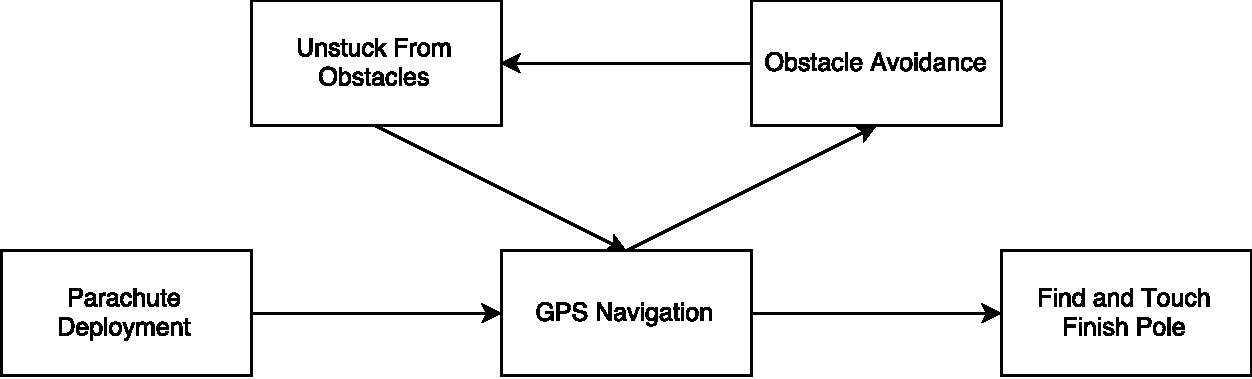
\includegraphics[page=1, scale=0.5]{flowchart.pdf}
  \end{tabular}
\end{figure}

The first thing the program starts is the parachute deployment module. Once on the ground, the GPS Navigation Module starts, which begins moving the rover in the direction of the finish. Next, the Obstacle Avoidance Module runs to navigate around any obstacles. If the rover detects that it has gotten stuck, the Unstuck from Obstacles module will run next. Then, the GPS Navigation module will run again to correct course. These three modules will continue to run in a loop until the rover is within the GPS error range of the finish coordinates, the control will switch to the Find and Touch the Finish Pole module, which will complete the rover's task and end the program.\vspace{.3cm}

\subsection{\textbf{Hardware Requirements}}
This software is meant to run on a Raspberry Pi Zero running Linux fitted with a custom PCB board to house the GPS sensor and control the various motors and servos attached to it. The only hardware this software will run on correctly is the custom built Rover designed by the ECE and ME teams. A version of the software is available which doesn't include the software to control the motors and sensors, though, which can be run on any Linux system with a camera.\vspace{.3cm}

\subsection{\textbf{Installation}}
\subsubsection{\textbf{Prerequisites}}
In order to install the testing version of this software, which doesn't include code to obtain data from the GPS or move the various motors and servos attached to the rover, a Linux system with OpenCV 2.4.9 is required. Additionally, to run on the actual hardware, wiringPi must be installed as well, which is a PIN based GPIO access library for the Raspberry Pi.\vspace{.3cm}

\subsubsection{\textbf{Compile and Run}}
To compile, simply run the makefile located in the final directory. To run the test version on any machine type make test with the DEBUG variable set to 1 in main.h. To run on the actual satellite hardware type make final with the DEBUG variable set to 0 (by default set to test version with DEBUG = 1). When run on the actual hardware, there will be no way to access the operating system to run the program, so use Crontab to run the program automatically after booting.


\section{\textbf{Resources}}
\subsection{\textbf{Machine Learning}}
Machine learning was a difficult was a difficult aspect of this project. I would not have been able to accomplish what I did without the assistance of Professor Bill Smart and his graduate students, as well as, without a few notable online resources. Bill Smart put me in contact with several of his graduate students who were able to point me in the right direction with various resources, and they were able to find a flaw in my settings which allowed me to eventually complete the training of my Haar classifier.\vspace{.3cm}
\par
Bill Smart has his PhD in Computer Science and a Masters in Intelligent Robotics. His research is focused in the areas of robotics and machine learning so he one of the most valuable resources in the world on the particular topic.\vspace{.3cm}
\par
Bill Smart\par
Associate Professor of Mechanical Engineering\par
Office: 316 Graf Hall\par
Phone: (541)905-2553
Email: bill.smart@oregonstate.edu\vspace{.3cm}
\par
If you are new to machine learning, or new to training a Haar classifier then you should surely download the haartraining toolkit from the following website. This kit comes with some instructions on training your haar classifier, but I found it most useful for the opencv-haar-cascade-positive-image-builder tool. If you only have time or the resources to come up with a limited number of images which have the object you are trying to detect in them, then this tool will help create additional images. For a strong classifier you will need hundreds, maybe thousands of images which have the object in them. What this tool will do is it will turn each image into many images by rotating it along different axis and changing the lighting.\vspace{.3cm}
\par 
 http://www.tectute.com/2011/06/opencv-haartraining.html\vspace{.3cm}
\par
Here are a couple websites which have useful tutorials:\vspace{.3cm}
\par
http://memememememememe.me/post/training-haar-cascades/
\par
http://coding-robin.de/2013/07/22/train-your-own-opencv-haar-classifier.html\vspace{.3cm}
\par
This next link is to an amazing video tutorial which I followed almost directly:\vspace{.3cm}
\par
https://www.youtube.com/watch?v=KFC6jxBKtBQ\vspace{.3cm}
\par
All computer vision software which I wrote uses the OpenCV library. OpenCV stands for Open Source Computer Vision. The OpenCV project has amazing documentation for everything you can do with their library. Below is the link to the OpenCV Cascade Classifier page which has the program which I used as my driver to test my Haar classifer. There are many resources here when working on computer vision.\vspace{.3cm}
\par   
http://docs.opencv.org/2.4/doc/tutorials/objdetect/cascade\_classifier/cascade\_classifier.html\#cascade-classifier

\section{\textbf{What We Learned}}

\subsection{\textbf{Zachary DeVita}}

\subsection{\textbf{Paul Minner}}

\subsection{\textbf{Steven Silvers}}

\subsection{\textbf{Zhaolong Wu}}






\section{\textbf{Appendix I: Essential Code}}
Computer vision provides an integral component in the success of the rover on its expedition. There are two separate and distinct functions which are performed using computer vision. While the rover is being directed by the GPS, computer vision will be used to detect obstacles in the path of the rover. This is accomplished by using a series of filters which are primarily intended to eliminate noise and to detect the edges of the obstacles. The other function of the computer vision is to identify the orange traffic cone. Our team has developed a complex system which utilizes machine learning and image processing to carry out this task.\vspace{.3cm}
\par
\subsection{\textbf{Obstacle Avoidance}}
The obstacle detection algorithm our team has implemented requires that each frame recorded by the camera is run through a series of filters which are intended to eliminate noise in the image and to detect the edges of the obstacles in the rover's path. Below is the algorithm which has been developed.\vspace{.3cm}
\par
\begin{minipage}{\textwidth}
\begin{lstlisting}
/** @function checkObstacle */
void Obstacle::checkObstacle()
{
	Mat frame, blurred, gray, canny;

	if (!DEBUG) {
		//Capture frame from camera
		VideoCapture capture(0);
		capture >> frame;
	}
	cvtColor(frame, gray, CV_BGR2GRAY);
	blur(gray, blurred, Size(40, 4));

	//	Morphological opening (remove small objects from the foreground)
	erode(blurred, blurred, getStructuringElement(MORPH_RECT, Size(5, 5)));
	dilate(blurred, blurred, getStructuringElement(MORPH_RECT, Size(5, 5)));
	dilate(blurred, blurred, getStructuringElement(MORPH_RECT, Size(5, 5)));

	Canny(blurred, canny, 50, 120, 3);

	int Image_Array[Width][Height];
	for(int i=0; i<canny.rows; i++)
		{
			for(int j=0; j<canny.cols; j++)
				{
					Vec3b color = canny.at<Vec3b>(Point(j,i));
					if(color.val[0] >= 25 && color.val[1] >= 25 && color.val[2] >= 25) {
						Image_Array[j][i] = 1;
					}
					else {
						Image_Array[j][i] = 0;
					}
				}
		}
	//start of obstacle avoidance section
	Analyze(Image_Array, Width, Height);
}
\end{lstlisting}
\end{minipage}
\par
As for an explanation, the VideoCapture constructor opens the video capture device and records a single frame from the camera. This data gets stored in a Mat (i.e. matrix) object each time this function is called. The cvtColor() function converts the frame to its equivalent in grayscale, and this gets stored in a separate Mat object. The blur() function does exactly what it sounds like; it blurs the frame using a specified parameter which has been determined through testing. Next, the now blurred, grayscale frame is put through a morphological transformation. The final filter used is the Canny Edge detection algorithm. The Canny algorithm is an extremely complex algorithm that I could write a book explaining so I will explain what it does opposed to how it works. The Canny algorithm is used to filter out any noise left in the image. The algorithm finds all edges in the image and uses the smallest value between thresholds for edge linking. The largest values are used to find initial segments of strong edges \cite{opencv2}. The set of nested loops is used to store the results from the Canny Edge detection algorithm into a double array containing 1s and 0s depending on if the individual pixel represents an edge of an object in the frame or not.

\subsection{\textbf{Traffic Cone Detection}}
The algorithm implemented for detecting the traffic cone at the base of the pole is a complex system which utilizes machine learning, as well as, some image processing filters. For the machine learning, our team has trained a Haar Classifier which can be used to detect a traffic cone based on its features and geometry. Though effective at only detecting a traffic cone the majority of the time, machine learning classifiers are prone to returning false positives. The way we have avoided this is by verifying the results by confirming that the color of the result is orange.\vspace{.3cm}
\par 
The way the color is checked is that several points from the potential result, i.e. pixels, are converted to their HSV (Hue, Saturation \& Value) equivalent, and are then compared with values which would be typically observed on an orange traffic cone. If the HSV values cannot be confirmed, then the image is rejected. This results in a higher rate of false negatives, but it also ensures that the results are accurate. Below is the algorithm which has been developed.

\clearpage
\begin{minipage}{\textwidth}
\begin{lstlisting}
/** @function detectAndDisplay */
int Finish::detectAndDisplay(Mat frame) {
	std::vector<Rect> cones;
	Mat gray;
	int quintant = 0;

	cvtColor(frame, gray, COLOR_BGR2GRAY);
	equalizeHist(gray, gray);

	//-- Detect cones
	cone_cascade.detectMultiScale(gray, cones, 1.1, 2, 0 | CASCADE_SCALE_IMAGE, Size(30, 30));

	if (cones.size() != 1)
		return 0;

	if (!isOrange(frame, cones[0])) {
		return 0;
	}

	rectangle(frame, Point(cones[0].x, cones[0].y), Point(cones[0].x + cones[0].width, cones[0].y + cones[0].height), Scalar(255, 255, 255), 2, 8);
	Point target(cones[0].x + cones[0].width / 2, cones[0].y + cones[0].height * 0.8);
	circle(frame, target, 3, Scalar(101, 255, 0), -1, 8);

	imshow("FRAME", frame);

	return selectQuintant(frame.size().width, target.x);
}
\end{lstlisting}
\end{minipage}
\par
As for an explanation, the above function takes a video frame from the camera sensor and converts it to grayscale. The grayscale frame has its histogram equalized which essentially means that the brightness of the image is normalized and the contrast of the image is increased. The image is then scanned using the machine learning algorithm for traffic cones. If traffic cones are found, two catty-corner points are stored as a rectangle object in a vector. Then the object is sent to the isOrange() function to confirm the color is orange. Lines 20-24 in the function are purely used for displaying the result. This is useful for testing and showing the algorithm, but these lines will not be implemented in the rover. The final line of code simply calls a function which determines which of the five segments the center of the cone is located in.
\vspace{.3cm}
\par
\begin{minipage}{\textwidth}
\begin{lstlisting}
/** @function isOrange */
bool Finish::isOrange(Mat original, Rect cone) {
	Mat HSV;
	int xVal = cone.x + cone.width / 2;
	int yVal[3] = { 
		cone.y + cone.height*0.8, 
		cone.y + cone.height*0.2, 
		cone.y + cone.height*0.5 
	};
	
	for (int i = 0; i < sizeof(yVal)/sizeof(*yVal); ++i) {
		Mat RGB = original(Rect(xVal, yVal[i], 1, 1));
		cvtColor(RGB, HSV, CV_BGR2HSV);
		Vec3b hsv = HSV.at<Vec3b>(0, 0);
		int H = hsv.val[0];		//	Hue
		int S = hsv.val[1];		//	Saturation
		int V = hsv.val[2];		//	Value

		if (H < 180 && S > 39 && V > 234)
			return true;
	}
	return false;
}
\end{lstlisting}
\end{minipage}
\par
The above algorithm takes three points from the potential traffic cone result in the image. The three points are taken from the horizontal center of the rectangle object, and with y-values from near the top, another near the bottom, and another from the center of the object. The HSV values are taken from each point, and, if any one of the points turns out to be orange, then the function returns true.

\section{\textbf{Appendix II: }}


\section{References}

%\bibliographystyle{IEEEtran}
%\bibliography{prog3}

\end{document}
